\typeout{(body.tex)}

\begin{frame}
    \titlepage
\end{frame}
\usepgflibrary{shapes.gates.logic.mux}
\newcommand{\z}[2]{\only<#1->{\myemph<#1|handout:0>{#2}}}
\newcommand{\zz}[3]{\only<#1-#2|handout:0>{\myemph<#1|handout:0>{#3}}}
\newcommand{\zzx}[3]{\only<#1-#2|handout:0>{#3}}
\newlength{\oneZero}
\settowidth{\oneZero}{\small\tt 0}
\newlength{\twoZeroes}
\settowidth{\twoZeroes}{\small\tt 00}

\tikzset{
    matrix stages/.style={
        row 1 column 2/.append style={nodes={fill=yellow!20}},
        row 1 column 3/.append style={nodes={fill=orange!20}},
        row 1 column 4/.append style={nodes={fill=green!20}},
        row 1 column 5/.append style={nodes={fill=blue!20}},
        row 1 column 6/.append style={nodes={fill=violet!20}},
        nodes={text depth=0.2ex},
    },
    hiBox/.style={fill=red,opacity=0.2},
}

\lstset{language=C}

% FIXME: more complete explanation of exercise?
\usetikzlibrary{matrix,shapes.callouts,positioning,calc}
\begin{frame}<0>[fragile,label=pattern1]{example access pattern (1)}
\begin{tikzpicture}
\tikzset{
    v/.style={visible on=<#1->,alt=<#1>{red}},
    h/.style={alt=<#1>{red}},
}
\tikzset{
    tagColor/.style={color=green!60!black},
    dataColor/.style={color=blue!60!black},
    offsetColor/.style={color=yellow!30!black},
}
\matrix[tight matrix,
        nodes={font=\small,minimum height=.5cm,text depth=.1ex},
        column 1/.append style={nodes={font=\small\tt,text width=3.3cm,align=left}},
        row 1/.append style={nodes={font=\small\bfseries}},
        column 2/.append style={nodes={text width=1.3cm}},
        ] (pattern) {
    address (hex)\& result \\
    00000000 (00) \& |[v=4]| miss \\
    00000001 (01) \& |[v=5,h=12]| hit \\
    01100011 (63) \& |[v=6]| miss \\
    01100001 (61) \& |[v=7,h=12]| miss \\
    01100010 (62) \& |[v=8]| hit \\
    00000000 (00) \& |[v=9,h=12]| miss \\
    01100100 (64) \& |[v=10]| miss \\
};
\begin{pgfonlayer}{fg}
    \begin{visibleenv}<12-13>
        \node[my callout2=pattern-7-2.east,anchor=west] at ([xshift=1cm]pattern-7-2.east) {
            miss caused by \myemph{conflict}
        };
    \end{visibleenv}
\end{pgfonlayer}
\matrix[tight matrix,anchor=north west,
        nodes={font=\small\tt,text depth=.1ex,text height=1ex,minimum height=1cm},
        row 1/.append style={nodes={font=\small\bfseries,minimum height=.5cm}},
        column 1/.append style={nodes={draw=none,text width=1.2cm}},
        column 2/.append style={nodes={align=center,text width=1cm}},
        column 3/.append style={nodes={align=center,tagColor,text width=1.5cm}},
        column 4/.append style={nodes={text width=2.5cm,align=center,dataColor,
            text depth=2.3ex}},
        row 1 column 4/.append style={nodes={text depth=.1ex}},
        label={[font=\small]$2$ byte blocks, $4$ sets}] (cache) at ([xshift=.5cm]pattern.north east) {
    index \& valid \& tag \& value \\
    00 \& \zzx{1}{3}{0}\z{4}{1} \& \zz{4,5}{6}{00000}\zz{7}{8}{01100}\z{9}{00000} \& 
        \zz{4,5}{6}{mem[0x00] mem[0x01]}%
        \zz{7}{8}{mem[0x60] mem[0x61]}%
        \z{9}{mem[0x00] mem[0x01]}%
        \\
    01 \& \zzx{1}{5}{0}\z{6}{1} \& \z{6}{01100} \& \z{6}{mem[0x62] mem[0x63]} \\
    10 \& \zzx{1}{9}{0}\z{10}{1} \& \z{10}{01100} \& \z{10}{mem[0x64] mem[0x65]} \\
    11 \& 0 \& ~ \& ~ \\
};
\begin{visibleenv}<2->
    \node[anchor=north west,font=\small,align=left] (explain1) at ([yshift=-.5cm]pattern.south west) {
        $m = 8$ bit addresses \\ 
        $S=4=2^s$ sets \\
        $s=\myemph<2>{2}$ (set) index bits \\
    };
    \node[anchor=north west,font=\small,align=left] (explain2) at ([xshift=.5cm]explain1.north east) {
        $B=2=2^b$ byte block size \\
        $b=\myemph<2>{1}$ (block) offset bits \\
        $t = m - (s+b) = \myemph<2>{5}$ tag bits\\
    };
\end{visibleenv}
\begin{visibleenv}<3->
    \coordinate (tagTopLeft) at ([xshift=.1ex]pattern-2-1.north west);
    \coordinate (tagBottomLeft) at ([xshift=.1ex]pattern-8-1.south west);
    \coordinate (indexTopLeft) at ([xshift=5\oneZero]tagTopLeft);
    \coordinate (offsetTopLeft) at ([xshift=2\oneZero]indexTopLeft);
    \coordinate (offsetTopRight) at ([xshift=1\oneZero]offsetTopLeft);
    \coordinate (tagBottomRight) at (tagBottomLeft -| indexTopLeft);
    \coordinate (indexBottomRight) at (tagBottomLeft -| offsetTopLeft);
    \coordinate (offsetBottomRight) at (tagBottomLeft -| offsetTopRight);
    \fill[tagColor,opacity=0.3] (tagTopLeft) rectangle (tagBottomRight);
    \fill[offsetColor,opacity=0.3] (offsetTopLeft) rectangle (offsetBottomRight);
    \begin{scope}[every node/.style={anchor=north,text depth=.2ex,text height=1ex}]
        \node[tagColor,xshift=-.5cm] at ($(tagBottomLeft)!.5!(tagBottomRight)$) {
            tag
        };
        \node[xshift=-.2cm] at ($(tagBottomRight)!.5!(indexBottomRight)$) {
            index
        };
        \node[offsetColor,xshift=.6cm] at ($(indexBottomRight)!.5!(offsetBottomRight)$) {
            offset
        };
    \end{scope}
\end{visibleenv}

\end{tikzpicture}
\end{frame}


\begin{frame}[fragile,label=pattern1Ex]{exercise}
\begin{tikzpicture}
\tikzset{
    v/.style={visible on=<#1->,alt=<#1>{red}},
    h/.style={alt=<#1>{red}},
}
\tikzset{
    tagColor/.style={color=green!60!black},
    dataColor/.style={color=blue!60!black},
    offsetColor/.style={color=yellow!30!black},
}
\matrix[tight matrix,
        nodes={font=\small,minimum height=.5cm,text depth=.1ex},
        column 1/.append style={nodes={font=\small\tt,text width=3.3cm,align=left}},
        row 1/.append style={nodes={font=\small\bfseries}},
        column 2/.append style={nodes={text width=1.3cm}},
        ] (pattern) {
    address (hex)\& result \\
    00000000 (00) \& ~ \\
    00000001 (01) \& ~ \\
    01100011 (63) \& ~ \\
    01100001 (61) \& ~ \\
    01100010 (62) \& ~ \\
    00000000 (00) \& ~ \\
    01100100 (64) \& ~ \\
};
\matrix[tight matrix,anchor=north west,
        nodes={font=\small\tt,text depth=.1ex,text height=1ex,minimum height=1cm},
        row 1/.append style={nodes={font=\small\bfseries,minimum height=.5cm}},
        column 1/.append style={nodes={draw=none,text width=1.2cm}},
        column 2/.append style={nodes={align=center,text width=1cm}},
        column 3/.append style={nodes={align=center,tagColor,text width=1.5cm}},
        column 4/.append style={nodes={text width=5cm,align=center,dataColor,
            text depth=2.3ex}},
        row 1 column 4/.append style={nodes={text depth=.1ex}},
        label={[font=\small]$4$ byte blocks, $4$ sets}] (cache) at ([xshift=.5cm]pattern.north east) {
    index \& valid \& tag \& value \\
    00 \& ~ \& ~ \& ~ \\
    01 \& ~ \& ~ \& ~ \\
    10 \& ~ \& ~ \& ~ \\
    11 \& ~ \& ~ \& ~ \\
};
\begin{visibleenv}<2>
    \node[draw=red,very thick,anchor=north west,align=left] (ex1) at ([yshift=-.5cm]pattern.south west) {
        how is the 8-bit address 61 (01100001) split \\ 
        up into tag/index/offset? 
    };
    \node[anchor=north west,align=left,font=\small] at (ex1.north east) {
        $b$ block offset bits;\\
        $B=2^b$ byte block size; \\
        $s$ set index bits; $S=2^s$ sets ;\\
        $t=m-(s+b)$ tag bits (leftover)
    };
\end{visibleenv}
\begin{visibleenv}<3-4>
\iftoggle{heldback}{}{
    \node[anchor=north west,font=\small,align=left] (explain1) at ([yshift=-.5cm]pattern.south west) {
        $m = 8$ bit addresses \\ 
        $S=4=2^s$ sets \\
        $s=\myemph<2>{2}$ (set) index bits \\
    };
    \node[anchor=north west,font=\small,align=left] (explain2) at ([xshift=.5cm]explain1.north east) {
        $B=4=2^b$ byte block size \\
        $b=\myemph<2>{2}$ (block) offset bits \\
        $t = m - (s+b) = \myemph<2>{4}$ tag bits\\
    };
}
\end{visibleenv}
\begin{visibleenv}<5>
    \node[anchor=north west,draw=red,very thick,align=left] at ([yshift=-.5cm]pattern.south west) {
        exercise: which accesses are hits?
    };
\end{visibleenv}
\begin{visibleenv}<4->
\iftoggle{heldback}{}{
    \coordinate (tagTopLeft) at ([xshift=.1ex]pattern-2-1.north west);
    \coordinate (tagBottomLeft) at ([xshift=.1ex]pattern-8-1.south west);
    \coordinate (indexTopLeft) at ([xshift=4\oneZero]tagTopLeft);
    \coordinate (offsetTopLeft) at ([xshift=2\oneZero]indexTopLeft);
    \coordinate (offsetTopRight) at ([xshift=2\oneZero]offsetTopLeft);
    \coordinate (tagBottomRight) at (tagBottomLeft -| indexTopLeft);
    \coordinate (indexBottomRight) at (tagBottomLeft -| offsetTopLeft);
    \coordinate (offsetBottomRight) at (tagBottomLeft -| offsetTopRight);
    \fill[tagColor,opacity=0.3] (tagTopLeft) rectangle (tagBottomRight);
    \fill[offsetColor,opacity=0.3] (offsetTopLeft) rectangle (offsetBottomRight);
    \begin{scope}[every node/.style={anchor=north,text depth=.2ex,text height=1ex}]
        \node[tagColor,xshift=-.5cm] at ($(tagBottomLeft)!.5!(tagBottomRight)$) {
            tag
        };
        \node[xshift=-.2cm] at ($(tagBottomRight)!.5!(indexBottomRight)$) {
            index
        };
        \node[offsetColor,xshift=.6cm] at ($(indexBottomRight)!.5!(offsetBottomRight)$) {
            offset
        };
    \end{scope}
}
\end{visibleenv}
\end{tikzpicture}
\end{frame}


\againframe<13>{pattern1}

% FIXME:
    % label ways
    % label parts in tag-split diagram or drop it
    % FIXME: MUXes not tall enough?
\usetikzlibrary{arrows.meta,calc,fit,positioning,matrix,circuits.logic.US,shapes.callouts}
\begin{frame}<1-3,12,4->[fragile,label=assocPattern]{adding associativity}
\tikzset{
    v/.style={visible on=<#1->,alt=<#1>{red}},
    h/.style={alt=<#1>{red}},
    tagColor/.style={color=green!60!black},
    dataColor/.style={color=blue!60!black},
    offsetColor/.style={color=yellow!30!black},
}

\begin{tikzpicture}
\matrix[tight matrix,
        nodes={font=\small\tt,text depth=.1ex,text height=1ex,minimum height=1cm},
        row 1/.append style={nodes={font=\small\bfseries,minimum height=.5cm}},
        column 1/.append style={nodes={draw=none,text width=1.2cm}},
        column 2/.append style={nodes={align=center,text width=1cm}},
        column 3/.append style={nodes={align=center,tagColor,text width=1.5cm}},
        column 4/.append style={nodes={text width=2.5cm,align=center,dataColor,
            text depth=2.3ex}},
        column 5/.append style={nodes={draw=none,text width=.1cm}},
        column 6/.append style={nodes={align=center,text width=1cm}},
        column 7/.append style={nodes={align=center,tagColor,text width=1.5cm}},
        column 8/.append style={nodes={text width=2.5cm,align=center,dataColor,
            text depth=2.3ex}},
        row 1 column 4/.append style={nodes={text depth=.1ex}},
        row 1 column 8/.append style={nodes={text depth=.1ex}},
        label={[font=\small]$2$-way set associative, $2$ byte blocks, $2$ sets}] (cache)  {
index \& valid \& tag \& value \& ~ \& valid \& tag \& value \\
0\&
    % i 0, 0:
    \zzx{1}{4}{0}\z{5}{1} \& 
    \z{5}{000000} \& 
    \z{5}{mem[0x00] mem[0x01]}  \& ~ \&
    % i 0, 1:
    \zzx{1}{7}{0}\z{8}{1} \& 
    \z{8}{011000} \& 
    \z{8}{mem[0x60] mem[0x61]} \\
1\& 
    % i 1, 0:
    \zzx{1}{6}{0}\z{7}{1} \& 
    \z{7}{011000} \&
    \z{7}{mem[0x62] mem[0x63]} \& ~ \&
    % i 1, 1:
    0 \& ~ \& ~ \\
};

\begin{visibleenv}<1|handout:0>
    \node[below=1cm of cache,align=left,draw=red,very thick] {
        multiple places to put values with same index \\
        avoid conflict misses
    };
\end{visibleenv}

\begin{visibleenv}<5-|handout:2>
    \matrix[tight matrix,anchor=north west,
            nodes={font=\small,minimum height=.5cm,text depth=.1ex},
            column 1/.append style={nodes={font=\small\tt,text width=3.3cm,align=left}},
            row 1/.append style={nodes={font=\small\bfseries}},
            column 2/.append style={nodes={text width=1.3cm}},
            ] (pattern) at ([yshift=-.5cm]cache.south west) {
        address (hex)\& result \\
        00000000 (00) \& |[v=5]| miss \\
        00000001 (01) \& |[v=6]| hit \\
        01100011 (63) \& |[v=7]| miss \\
        01100001 (61) \& |[v=8]| miss \\
        01100010 (62) \& |[v=9]| hit \\
        00000000 (00) \& |[v=10]| hit \\
        01100100 (64) \& |[v=11]| miss \\
    };
    \coordinate (tagTopLeft) at ([xshift=.1ex]pattern-2-1.north west);
    \coordinate (tagBottomLeft) at ([xshift=.1ex]pattern-8-1.south west);
    \coordinate (indexTopLeft) at ([xshift=6\oneZero]tagTopLeft);
    \coordinate (offsetTopLeft) at ([xshift=1\oneZero]indexTopLeft);
    \coordinate (offsetTopRight) at ([xshift=1\oneZero]offsetTopLeft);
    \coordinate (tagBottomRight) at (tagBottomLeft -| indexTopLeft);
    \coordinate (indexBottomRight) at (tagBottomLeft -| offsetTopLeft);
    \coordinate (offsetBottomRight) at (tagBottomLeft -| offsetTopRight);
    \fill[tagColor,opacity=0.3] (tagTopLeft) rectangle (tagBottomRight);
    \fill[offsetColor,opacity=0.3] (offsetTopLeft) rectangle (offsetBottomRight);
    \begin{scope}[every node/.style={anchor=north,text depth=.2ex,text height=1ex}]
        \node[tagColor,xshift=-.5cm] at ($(tagBottomLeft)!.5!(tagBottomRight)$) {
            tag
        };
        \node[xshift=-.2cm] at ($(tagBottomRight)!.5!(indexBottomRight)$) {
            index
        };
        \node[offsetColor,xshift=.6cm] at ($(indexBottomRight)!.5!(offsetBottomRight)$) {
            offset
        };
    \end{scope}
\end{visibleenv}

\begin{visibleenv}<11>
    \node[my callout2=pattern-8-2.east,anchor=west] at ([xshift=-1cm,yshift=1.2cm]pattern-8-2.east) { 
        needs to replace block in set 0!
    };
    \node[inner sep=-1pt,draw=red,line width=2pt,fit=(cache-2-2) (cache-2-8)] {};
\end{visibleenv}

\begin{visibleenv}<2>
    \node[inner sep=-1pt,draw=red,line width=2pt,fit=(cache-2-2) (cache-2-8),
        label={[red,xshift=-1cm,font=\bfseries]center:set 0}] {};
    \node[inner sep=-1pt,draw=red,line width=2pt,fit=(cache-3-2) (cache-3-8),
        label={[red,xshift=-1cm,font=\bfseries]center:set 1}] {};
\end{visibleenv}

\begin{visibleenv}<3>
    \node[inner sep=-1pt,draw=orange,line width=2pt,fit=(cache-2-2) (cache-3-4),
        label={[orange,font=\bfseries,fill=white]center:way 0}] {};
    \node[inner sep=-1pt,draw=orange,line width=2pt,fit=(cache-2-6) (cache-3-8),
        label={[orange,font=\bfseries,fill=white]center:way 1}] {};
\end{visibleenv}

\begin{visibleenv}<4|handout:2>
    \node[anchor=north west,font=\small,align=left] (explain1) at ([yshift=-.5cm]cache.south west) {
        $m = 8$ bit addresses \\ 
        $S=2=2^s$ sets \\
        $s=\myemph<2>{1}$ (set) index bits \\
    };
    \node[anchor=north west,font=\small,align=left] (explain2) at ([xshift=.5cm]explain1.north east) {
        $B=2=2^b$ byte block size \\
        $b=\myemph<2>{1}$ (block) offset bits \\
        $t = m - (s+b) = \myemph<2>{6}$ tag bits\\
    };
\end{visibleenv}

\end{tikzpicture}
\end{frame}

\begin{frame}{cache operation (associative)}
\begin{tikzpicture}[circuit logic US]
\tikzset{
    myline/.style={-latex,thick},
    myline thin/.style={-latex,thin},
    myline bus/.style={-latex,ultra thick},
    myline no arrow/.style={thick},
    offsetColor/.style={color=yellow!30!black},
    tagColor/.style={color=green!60!black},
    tagStoreFill/.style={fill=green!20},
    tagColorFill/.style={tagColor,fill=green!60!black},
    dataColor/.style={color=blue!60!black},
    dataColorFill/.style={tagColor,fill=blue!60!black},
    dataStoreFill/.style={fill=blue!20},
    triangle down/.style = {draw,regular polygon, regular polygon sides=3, shape border rotate=180},
}
\matrix[tight matrix,
        nodes={draw,
               font=\small\tt,
               text depth=0.2ex,
               text height=1.4ex,
        },
        row 1/.style={nodes={font=\small\bfseries}},
        column 1/.style={nodes={text width=1cm,align=center}},
        column 2/.style={nodes={text width=1cm,tagColor,tagStoreFill}},
        column 3/.style={nodes={text width=1.3cm,dataColor,dataStoreFill}},
        column 4/.style={nodes={text width=.1cm,draw=none}},
        column 5/.style={nodes={text width=1cm,align=center}},
        column 6/.style={nodes={text width=1cm,tagColor,tagStoreFill}},
        column 7/.style={nodes={text width=1.3cm,dataColor,dataStoreFill}},
        ] (cache) {
    valid \& tag \&  data \& ~ \& valid \& tag \& data\\
    1  \& 10 \& 00 11 \& ~ \& 1 \& 00 \& AA BB \\
    ~ \& ~ \& ~ \&   ~ \&  ~ \& ~ \& ~\\
    ~ \& ~ \& ~ \&   ~ \&  ~ \& ~ \& ~\\
    ~ \& ~ \& ~ \&   ~ \&  ~ \& ~ \& ~\\
    1 \&  11 \& B4 B5 \& ~ \& 1 \& 01 \& 33 44 \\
    ~ \& ~ \& ~ \&   ~ \&  ~ \& ~ \& ~\\
    ~ \& ~ \& ~ \&   ~ \&  ~ \& ~ \& ~\\
    ~ \& ~ \& ~ \&   ~ \&  ~ \& ~ \& ~\\
};
\begin{scope}[every node/.style={draw,rectangle,dashed,inner xsep=0pt,outer sep=0pt,font=\tt}]
\node (idx) at ([yshift=.5cm,xshift=-.3cm]cache.north west){100};
\node[left=0cm of idx,tagColor] (tag) {11};
\node[right=0cm of idx,offsetColor] (offset) {1};
\end{scope}
\draw[thick,dashed,-latex] (idx) |- (cache-6-1.west) node[near start,font=\small,fill=white,inner sep=2pt,xshift=-.3cm] {index};

%\begin{visibleenv}<2->
    \node[below=0.3cm of cache-9-2,draw,circle,inner sep=3pt] (comp1) {\small =};
    \node[below=1.4cm of cache-9-6,draw,circle,inner sep=3pt] (comp2) {\small =};
    %\coordinate(comp1Intersect) at ($(comp1) + (-.7cm,0.5cm)$);
    %\node[draw,circle,tagColorFill,inner sep=0pt,minimum width=1mm] at (comp1Intersect) {};
    \draw[tagColor,myline] (cache-9-2) -- (comp1);
    \draw[tagColor,myline] (cache-9-6) -- (comp2);

    %\draw[myline no arrow,tagColor] (tag) |- (comp1Intersect);
    %\draw[myline,tagColor] (comp1Intersect) |- (comp1);
    \draw[tagColor,myline] (tag) |- (comp2);
    \draw[tagColor,myline] (tag) |- (comp1) node[near start,font=\small,fill=white] {tag};
    %\draw[myline no arrow,tagColor] (comp1Intersect) |- (comp2Intersect);
    %\draw[myline,tagColor] (comp2Intersect) |- (comp2);

    \node[xshift=-.4cm,draw,below=1cm of cache-9-3,and gate,logic gate inputs=nn,label={[font=\scriptsize]center:AND}] (validCheck1) {};
    \node[xshift=-.4cm,draw,below=2.0cm of cache-9-7,and gate,logic gate inputs=nn,label={[font=\scriptsize]center:AND}] (validCheck2) {};
    \draw[myline] (comp1.south) |- (validCheck1.input 1);
    \draw[myline] (cache-9-1.south) |- (validCheck1.input 2);
    \draw[myline] (comp2.south) |- (validCheck2.input 1);
    \draw[myline] (cache-9-5.south) |- (validCheck2.input 2);
%\end{visibleenv}

\node[fit=(cache-6-1) (cache-6-7),inner sep=1pt,red,draw,line width=3pt] {};

%\node[draw,trapezium,inner xsep=0pt,outer sep=0pt,trapezium angle=75,below=.7cm of validCheck2,
%text width=5cm,shape border rotate=180,xshift=1.5cm] (mux) {};
%\draw[myline] (validCheck1.output) -| (buffer1.west);
%\draw[myline] (cache-9-3.south) -- (buffer1);
%\draw[myline] (buffer1.south) -- (bufEnd1);
\coordinate (outputData) at ([xshift=1.5cm,yshift=-.5cm]cache-9-7.south east);
\coordinate (beforeOutputData) at ([xshift=-.5cm]outputData);
\coordinate (outputHit1) at ([xshift=-1.5cm] beforeOutputData |- validCheck1.output);
\coordinate (outputHit2) at ([xshift=-1.5cm] beforeOutputData |- validCheck2.output);
%\begin{visibleenv}<2->
\node[or gate,logic gate inputs=nn,label={[font=\scriptsize]center:OR},anchor=output] (validCheckTotal)
    at ([xshift=1cm]$(outputHit1)!0.5!(outputHit2)$) {};
%\draw[myline] (validCheck1.output) -- (outputHit1) |- (validCheckTotal.input 1);
    \draw[myline no arrow] (validCheck1.output) -- ([xshift=-1pt]validCheck1.output -| cache-9-5.south);
    \draw[myline no arrow] ([xshift=1pt]validCheck1.output -| cache-9-5.south) -- 
                  ([xshift=-2pt]validCheck1.output -| cache-9-6.south);
    \draw[myline no arrow] ([xshift=2pt]validCheck1.output -| cache-9-6.south) -- (outputHit1);
    \draw[myline] (outputHit1) |- (validCheckTotal.input 1);
\draw[myline] (validCheck2.output) -- (outputHit2) |- (validCheckTotal.input 2);
\draw[myline] (validCheckTotal.output) -- ++(.5cm,0cm) node[right] {is hit? ({\tt 1})};
%\end{visibleenv}
%\begin{visibleenv}<3->
    \node[dataColor,draw,minimum width=.5cm,minimum height=1cm,mux,anchor=east,inputs=nn] (outputSelect) at ([xshift=-.2cm]beforeOutputData) {};
    \draw[myline] (outputHit1) -| (outputSelect.south);
    \fill[black] (outputHit1) circle (2pt);
    %\draw[myline,dataColor] (cache-9-3.south) |- (outputSelect.input 2);
        \draw[dataColor,myline no arrow] (cache-9-3.south) |- ([xshift=-1pt]cache-9-5.south |- outputSelect.input 2);
        \draw[dataColor,myline no arrow] ([xshift=1pt]cache-9-5.south |- outputSelect.input 2) --
                               ([xshift=-1pt]cache-9-6.south |- outputSelect.input 2);
        \draw[dataColor,myline] ([xshift=1pt]cache-9-6.south |- outputSelect.input 2) --
                               (outputSelect.input 2);
    \draw[myline,dataColor] (cache-9-7.south) |- (outputSelect.input 1);
    \draw[myline no arrow,dataColor] (outputSelect.output) -- (beforeOutputData);
    \node[draw,minimum width=.5cm,minimum height=1cm,mux,anchor=west,inputs=nn] (selectByte) at (outputData) {};
    \foreach \x in {1,2} {
        \draw[dataColor,myline thin] (beforeOutputData) |- (selectByte.input \x);
    };
    \draw[offsetColor,myline] (offset.east) -| (selectByte.north) node[very near start,fill=white,font=\small] {offset};
    \draw[dataColor,myline thin] (selectByte.output) -- ++(0.5cm,0cm) -- ++(0cm,0.5cm) node[above,align=center] {data\\({\tt B5})};
%\end{visibleenv}

\begin{visibleenv}<2-3>
\node[draw,red,thick,fit=(validCheck1)] {};
\node[draw,red,thick,fit=(comp1)] {};
\draw[red,thick,dashed,-Latex] (validCheck1.output) -| (outputSelect.south);
\end{visibleenv}
\begin{visibleenv}<3>
\draw[thick,red,-Latex] (outputSelect.input 2) -- (outputSelect.output);
\end{visibleenv}
\end{tikzpicture}
% FIXME: place diagram here
\end{frame}

% FIXME: drop slide?
\begin{frame}{associative lookup possibilities}
    \begin{itemize}
    \item none of the blocks for the index are valid
    \item none of the valid blocks for the index match the tag
        \begin{itemize}
        \item something else is stored there
        \end{itemize}
    \item one of the blocks for the index is valid and matches the tag
    \end{itemize}
\end{frame}


\begin{frame}{associativity terminology}
\begin{itemize}
\item \myemph{direct-mapped} --- one block per set
\item \myemph{$E$-way set associative} --- $E$ blocks per set
    \begin{itemize}
    \item $E$ ways in the cache
    \end{itemize}
\item \myemph{fully associative} --- one set total (everything in one set)
\end{itemize}
\end{frame}


\begin{frame}{Tag-Index-Offset formulas (complete)}
\def\arraystretch{1.5}
\begin{tabular}{ll}
$m$ & memory addreses bits (Y86-64: 64) \\
$E$ & number of blocks per set (``ways'') \\
$S=2^s$ & number of sets \\
$s$  & (set) index bits \\
$B=2^b$ & block size \\
$b$ & (block) offset bits \\
$t = m - (s+b)$ & tag bits \\
$C = B \times S \times E$ & cache size (excluding metadata) \\
\end{tabular}
\end{frame}


\providecommand{\KB}{\text{KB}}
\providecommand{\Byte}{\text{Byte}}

\begin{frame}{T-I-O exercise: L1}
\iftoggle{heldback}{}{
\def\arraystretch{1.1}
\begin{tabular}{llll}
quantity & value for L1\\\hline
block size (given) & $B=64\Byte$  \\ \hline
           & \multicolumn{3}{l}{$B=2^b$ ($b$: block offset bits)} \\ \pause
block offset bits & $b=\myemph{6}$ \\ \hline \pause
blocks/set (given) & $E=8$ \\ \hline
cache size (given) & $C = 32\KB = E \times B \times S$ \\ \hline \pause
           & \multicolumn{3}{l}{$S = \frac{C}{B\times E}$ ($S$: number of sets)} \\\pause
number of sets & $S = \frac{32\KB}{64\Byte\times 8} = \myemph{64}$ \\\hline \pause
               & \multicolumn{3}{l}{$S = 2^s$ ($s$: set index bits)} \\
set index bits & $s = \log_2(64) = \myemph{6}$ \\\hline
\end{tabular}
}
\end{frame}

\begin{frame}{T-I-O results}
\iftoggle{heldback}{}{
\begin{tabular}{llll}
~ & L1 & L2 & L3 \\ \hline
sets & 64 & 1024 & 8192 \\
block offset bits & 6 & 6 & 6 \\
set index bits & 6 & 10 & 13 \\
tag bits & \multicolumn{3}{c}{(the rest)} \\
\end{tabular}
}
\end{frame}

\begin{frame}{T-I-O: splitting}
\iftoggle{heldback}{}{
\begin{tabular}{llll}
~ & L1 & L2 & L3 \\ \hline
block offset bits & \myemph<1|handout:0>{6} & 6 & 6 \\
set index bits & 6 & 10 & 13 \\
tag bits & \multicolumn{3}{c}{(the rest)} \\
\end{tabular}
\begin{itemize}
\item {\tt 0x34567}:
\begin{tabular}{ccccc}
3 & 4 & 5 & 6 & 7 \\
\tt \myemph<4|handout:0>{0\myemph<7|handout:0>{011}} & \tt \myemph<4,5,7|handout:0>{0100} & 
\tt \myemph<3,5,7|handout:0>{0101} & 
\tt \myemph<3,5,7|handout:0>{01}\myemph<2|handout:0>{10} & 
\tt \myemph<2|handout:0>{0111} \\
\end{tabular}
\item bits 0-\myemph<1|handout:0>{5} (all offsets): {\tt \myemph<2>{100111}} = {\tt 0x27}
\only<3-4|handout:1>{
\item<3-> L1:
\begin{itemize}
    \item bits 6-11 (L1 set): {\tt \myemph<3>{01 0101}} = {\tt 0x15}
    \item bits 12- (L1 tag): \myemph<4>{\tt 0x34}
\end{itemize}
}
\only<5-6|handout:2>{
\item<5-> L2:
\begin{itemize}
    \item bits 6-15 (set for L2): {\tt \myemph<5>{01 0001 0101}} = {\tt 0x115}
    \item bits 16-: {\tt 0x3}
\end{itemize}
}
\only<7-|handout:3>{
\item<7-> L3:
\begin{itemize}
    \item bits 6-18 (set for L3): {\tt \myemph<7>{0 1101 0001 0101}} = {\tt 0xD15}
    \item bits 18-: {\tt 0x0} 
\end{itemize}
}
\end{itemize}
}
\end{frame}



\begin{frame}{cache miss types}
    \begin{itemize}
        \item \textit{compulsory} (or \textit{cold}) --- \myemph{first time} accessing something
            \begin{itemize}
            \item adding more sets or blocks/set wouldn't change
            \end{itemize}
        \item \textit{conflict} --- sets aren't big/flexible enough
            \begin{itemize}
            \item a fully-associtive (1-set) cache of the same size would have done better
            \end{itemize}
        \item \textit{capacity} --- cache was not big enough
    \end{itemize}
\end{frame}


\usetikzlibrary{arrows.meta,calc,fit,matrix,positioning,shapes.callouts}
\begin{frame}[fragile,label=replPolicies]{replacement policies}
\tikzset{
    v/.style={visible on=<#1->,alt=<#1>{red}},
    h/.style={alt=<#1>{red}},
    tagColor/.style={color=green!60!black},
    dataColor/.style={color=blue!60!black},
    offsetColor/.style={color=yellow!30!black},
}

\begin{tikzpicture}
\matrix[tight matrix,
        nodes={font=\small\tt,text depth=.1ex,text height=1ex,minimum height=1cm},
        row 1/.append style={nodes={font=\small\bfseries,minimum height=.5cm}},
        column 1/.append style={nodes={draw=none,text width=1.1cm}},
        column 2/.append style={nodes={align=center,text width=1cm}},
        column 3/.append style={nodes={align=center,tagColor,text width=1.3cm,
            font=\tt\fontsize{10}{11}\selectfont}},
        column 4/.append style={nodes={text width=1.9cm,align=center,dataColor,
            font=\tt\fontsize{10}{11}\selectfont,
            text depth=2.3ex}},
        column 5/.append style={nodes={draw=none,text width=.1cm}},
        column 6/.append style={nodes={align=center,text width=1cm}},
        column 7/.append style={nodes={align=center,tagColor,text width=1.3cm,
            font=\tt\fontsize{10}{11}\selectfont}},
        column 8/.append style={nodes={text width=1.9cm,align=center,dataColor,
            font=\tt\fontsize{10}{11}\selectfont,
            text depth=2.3ex}},
        column 9/.append style={nodes={draw=none,text width=.1cm}},
        row 1 column 4/.append style={nodes={text depth=.1ex}},
        row 1 column 8/.append style={nodes={text depth=.1ex}},
        column 10/.append style={nodes={visible on=<2->,align=center}},
        label={[font=\small]$2$-way set associative, $2$ byte blocks, $2$ sets}] (cache)  {
index \& valid \& tag \& value \& ~ \& valid \& tag \& value \& ~\& LRU\\
0\&
    % i 0, 0:
    1 \& 
    000000 \& 
    mem[0x00] mem[0x01] \& ~\&
    % i 0, 1:
    1 \& 
    011000 \& 
    mem[0x60] mem[0x61] \& ~ \& 1 \\
1\& 
    % i 1, 0:
    1 \& 
    011000 \&
    mem[0x62] mem[0x63] \&  ~ \&
    % i 1, 1:
    0 \& ~ \& ~ \&  ~\& 1
    \\
};
\matrix[tight matrix,anchor=north west,
            nodes={font=\small,minimum height=.5cm,text depth=.1ex},
            column 1/.append style={nodes={font=\small\tt,text width=3.3cm,align=left}},
            row 1/.append style={nodes={font=\small\bfseries}},
            column 2/.append style={nodes={text width=1.3cm}},
            ] (pattern) at ([yshift=-.5cm]cache.south west) {
        address (hex)\& result \\
        00000000 (00) \&  miss \\
        00000001 (01) \& hit \\
        01100011 (63) \& miss \\
        01100001 (61) \& miss \\
        01100010 (62) \&  hit \\
        00000000 (00) \& hit \\
        01100100 (64) \& |[red]| miss \\
    };
\node[inner sep=-1pt,draw=red,line width=2pt,fit=(cache-2-2) (cache-2-8)] {};
\begin{visibleenv}<1|handout:0>
    \node[my callout2=cache-2-4.south,anchor=north] at ([yshift=-2cm]cache-2-4.south) {
        how to decide where to insert 0x64?
    };
\end{visibleenv}
\begin{visibleenv}<2>
    \node[my callout2=cache-3-10.south,anchor=north,align=left] at ([yshift=-1cm,xshift=-1cm]cache-3-8.south) {
        track which block was read least recently \\
        updated on \myemph{every access}
    };
\end{visibleenv}
\end{tikzpicture}
\end{frame}

\begin{frame}{example replacement policies}
\begin{itemize}
    \item least recently used
        \begin{itemize}
        \item take advantage of \myemph{temporal locality}
        \item at least $\left\lceil\log_2(E!)\right\rceil$ bits per set for $E$-way cache
            \begin{itemize}
            \item (need to store order of all blocks)
            \end{itemize}
        \end{itemize}
    \item approximations of least recently used
        \begin{itemize}
        \item implementing least recently used is expensive --- lots of bookkeeping bits+time
        \item really just need ``avoid recently used'' --- much faster/simpler
        \item good approximations: $E$ to $2E$ bits
        \end{itemize}
    \item first-in, first-out
        \begin{itemize}
        \item counter per set --- where to replace next
        \end{itemize}
    \item (pseudo-)random
        \begin{itemize}
        \item no extra information!
        \item actually works pretty well in practice
        \end{itemize}
\end{itemize}
\end{frame}



\newcommand<>{\ans}[1]{%
    \iftoggle{heldback}{}{\only#2{#1}}%
}

\begin{frame}[fragile,label=pattern2Ex]{exercise}
\begin{tikzpicture}
\tikzset{
    v/.style={visible on=<#1->,alt=<#1>{red}},
    h/.style={alt=<#1>{red}},
}
\tikzset{
    tagColor/.style={color=green!60!black},
    dataColor/.style={color=blue!60!black},
    offsetColor/.style={color=yellow!30!black},
}
\matrix[tight matrix,
        nodes={font=\small,minimum height=.48cm,text depth=.1ex},
        column 1/.append style={nodes={font=\small\tt,text width=3.3cm,align=left}},
        row 1/.append style={nodes={font=\small\bfseries}},
        column 2/.append style={nodes={text width=1cm}},
        ] (pattern) {
    address (hex)\& hit?\\
    00000000 (00) \& |[v=5]| \only<5->{miss} \\
    00000001 (01) \& \ans<6->{hit} \\
    00001010 (0A) \& |[v=6]| \ans<6->{miss} \\
    00100001 (21) \& |[v=7]| \ans<7->{miss} \\
    00001100 (0C) \& \ans<7->{miss} \\
    00000011 (02) \& |[v=8]| \ans<8->{miss} \\
    00100011 (23) \& |[v=9]| \ans<9->{hit} \\
};
\matrix[tight matrix,anchor=south west,
        nodes={font=\small\tt,text depth=.1ex,text height=1ex,minimum height=1cm},
        row 1/.append style={nodes={font=\small\bfseries,minimum height=.5cm}},
        column 1/.append style={nodes={draw=none,text width=1.2cm}},
        column 2/.append style={nodes={align=center,text width=.5cm}},
        column 3/.append style={nodes={align=center,tagColor,text width=1.25cm}},
        column 4/.append style={nodes={text width=3.5cm,align=center,dataColor,
            text depth=2.3ex,font=\fontsize{10}{11}\selectfont}},
        column 5/.append style={nodes={draw=none,text width=0.25cm}},
        column 6/.append style={nodes={align=center,text width=.5cm}},
        column 7/.append style={nodes={align=center,tagColor,text width=1.25cm}},
        column 8/.append style={nodes={text width=3.5cm,align=center,dataColor,
            text depth=2.3ex,font=\fontsize{10}{11}\selectfont}},
        column 9/.append style={nodes={draw=none,text width=0.25cm}},
        column 10/.append style={nodes={text width=1cm,font=\fontsize{9}{10}\selectfont}},
        row 1 column 4/.append style={nodes={text depth=.1ex}},
        row 1 column 8/.append style={nodes={text depth=.1ex}},
        label={[overlay,font=\small]$4$ byte blocks, $2$ sets}] (cache) at ([yshift=.25cm]pattern.north west) {
            index \& V \& tag \& value \& ~ \& V \& tag \& value \& ~ \& LRU \\
    0 \& \only<1-4>{0}\only<5->{1} \& \only<5>{00000}\ans<6>{00000}\ans<7->{\myemph<7>{00100}} \& \only<5>{M[0x00] M[0x01] M[0x02] M[0x03]}\ans<6>{M[0x00] M[0x01] M[0x02] M[0x03]}\ans<7->{M[0x20] M[0x21] M[0x22] M[0x23]} \& ~
      \& \only<1-5>{0}\ans<6->{1} \& \ans<6-7>{00001}\ans<8->{\myemph<8>{00000}} \& \only<6-7>{M[0x08] M[0x09] M[0x0A] M[0x0B]}\ans<8->{M[0x00] M[0x01] M[0x02] M[0x03]}  \& ~ \& \only<5>{way 1}\ans<6>{way 0}\ans<7>{way 1}\ans<8>{way 0}\ans<9>{\myemph<9>{way 1}} \\
    1 \& \only<1-5>{0}\ans<6-7>{0}\ans<8->{1} \& \ans<8->{00000} \& \ans<8->{M[0x0C] M[0x0D] M[0x0E] M[0x0F]} \& ~  \& 0 \& ~ \& ~  \& ~ \& \ans<8->{way 1} \\
};
\begin{visibleenv}<2>
    \node[draw=red,very thick,anchor=north west,align=left] (ex1) at ([xshift=.5cm]pattern.north east) {
        how is the address 21 (00100001) split \\ 
        up into tag/index/offset? 
    };
    \node[anchor=north west,align=left,font=\small] at (ex1.south west) {
        $b$ block offset bits;\\
        $B=2^b$ byte block size; \\
        $s$ set index bits; $S=2^s$ sets;\\
        $t=m-(s+b)$ tag bits (leftover)
    };
\end{visibleenv}
\begin{visibleenv}<3->
\iftoggle{heldback}{}{
    \coordinate (tagTopLeft) at ([xshift=.1ex]pattern-2-1.north west);
    \coordinate (tagBottomLeft) at ([xshift=.1ex]pattern-8-1.south west);
    \coordinate (indexTopLeft) at ([xshift=5\oneZero]tagTopLeft);
    \coordinate (offsetTopLeft) at ([xshift=1\oneZero]indexTopLeft);
    \coordinate (offsetTopRight) at ([xshift=2\oneZero]offsetTopLeft);
    \coordinate (tagBottomRight) at (tagBottomLeft -| indexTopLeft);
    \coordinate (indexBottomRight) at (tagBottomLeft -| offsetTopLeft);
    \coordinate (offsetBottomRight) at (tagBottomLeft -| offsetTopRight);
    \fill[tagColor,opacity=0.3] (tagTopLeft) rectangle (tagBottomRight);
    \fill[offsetColor,opacity=0.3] (offsetTopLeft) rectangle (offsetBottomRight);
    \begin{scope}[every node/.style={anchor=north,text depth=.2ex,text height=1ex}]
        \node[tagColor,xshift=-.5cm] at ($(tagBottomLeft)!.5!(tagBottomRight)$) {
            tag
        };
        \node[xshift=-.2cm] at ($(tagBottomRight)!.5!(indexBottomRight)$) {
            index
        };
        \node[offsetColor,xshift=.6cm] at ($(indexBottomRight)!.5!(offsetBottomRight)$) {
            offset
        };
    \end{scope}
}
\end{visibleenv}
\begin{visibleenv}<4-5>
    \node[anchor=north west,draw=red,very thick,align=left] at ([xshift=.5cm]pattern.north east) {
        exercise: how many accesses are hits? \\
        what is the final state of the cache?
    };
\end{visibleenv}
\end{tikzpicture}
\end{frame}


\usetikzlibrary{arrows.meta,matrix,positioning,shapes.callouts,shapes.misc}
\begin{frame}{write-through v. write-back}
\begin{tikzpicture}
\tikzset{
    stepCircle/.style={circle,fill=yellow!10,draw,very thick,inner sep=1pt},
    every pin edge/.style={-,thick},
}

\node[draw,minimum width=1cm,minimum height=2.5cm] (cpu) {CPU};
\node[draw,minimum width=3cm,minimum height=4cm,right=4cm of cpu] (cache) {Cache};
    \node[above=2cm of cache,font=\bfseries] {
        \only<1-2>{option 1: write-through}\only<3-4>{option 2: write-back}
    };
\node[draw,minimum width=3cm,minimum height=6cm,right=4cm of cache] (mem) {RAM};
    \node[align=center,draw] (storedValue) at ([yshift=-1cm]cache.center) {{\tt ABCD}: \only<1>{FF}\only<2->{\myemph<2,3>{10}} \\ 
        \only<3->{(\myemph{dirty})}};
    \node[align=center,draw,anchor=north] (storedValueMem) at ([yshift=-.5cm]mem.center) {\ldots \\ {\tt 11CD}: {\tt 42} \\ {\tt ABCD}: \only<1,3>{FF}\only<2,4->{\myemph<4>{10}} \\ \ldots};

\begin{scope}[every node/.style={inner sep=1pt},every pin/.style={align=center}]
    \draw[very thick,-Latex] ([yshift=1cm]cpu.east) -- ([yshift=1cm]cache.west)
        node[-,midway,pin={[name=writeToCache]north:write {\tt 10}\\to {\tt 0xABCD}}] (cacheWrite) {};
    \node[stepCircle] at (writeToCache.north west) {1};
    \begin{visibleenv}<2>
        \draw[very thick,-Latex] ([yshift=1cm]cache.east) coordinate (cacheOut) --
            ([yshift=1cm]mem.west) coordinate (memIn)
            node[-,midway,pin={[name=forwardWrite]north:write {\tt 10}\\to {\tt 0xABCD}}] {};
        \node[stepCircle] at (forwardWrite.north west) {2};
    \end{visibleenv}
\end{scope}
\begin{visibleenv}<4->
    \node[draw,thick,cross out,minimum width=2cm,minimum height=1cm] at (storedValue) {};
\end{visibleenv}
\begin{visibleenv}<4->
    \node[pin={[align=center,name=readCmd]south:read \\ from \\ {\tt 0x11CD} \\ (conflicts)}] at (cacheWrite) {};
    \node[stepCircle] at (readCmd.north west) {2};
    \draw[very thick,-Latex] (cacheOut) -- (memIn)
        node[midway,pin={[align=center,name=writeBackOut]north:write {\tt 10} \\ to {\tt ABCD}}] {};
    \node[stepCircle] at (writeBackOut.north west) {3};
\end{visibleenv}
\begin{visibleenv}<4>
    \node[my callout2=storedValue.south,anchor=north] at ([yshift=-1cm]storedValue) {
        \ldots{} when replaced --- send value to memory
    };
\end{visibleenv}
\begin{visibleenv}<5->
    \path (cacheOut) -- (memIn)
        node[midway,pin={[align=center,name=actualRead]south:read\\from\\{\tt 0x11CD}}] {};
    \node[stepCircle] at (actualRead.north west) {4};
    \node[my callout2=actualRead.south,anchor=north] at ([xshift=1cm,yshift=-1cm]storedValue) {
        \ldots{} read new value to store in cache
    };
\end{visibleenv}
% FIXME: hilite hit miss in diagram, separate into animation
\end{tikzpicture}
\end{frame}

\begin{frame}[fragile,label=writebackBits]{writeback policy}
\begin{tikzpicture}
\tikzset{
    v/.style={visible on=<#1->,alt=<#1>{red}},
    h/.style={alt=<#1>{red}},
    tagColor/.style={color=green!60!black},
    dataColor/.style={color=blue!60!black},
    offsetColor/.style={color=yellow!30!black},
}
\matrix[tight matrix,
        nodes={font=\small\tt,text depth=.1ex,text height=1ex,minimum height=1cm},
        row 1/.append style={nodes={font=\small\bfseries,minimum height=.5cm}},
        column 1/.append style={nodes={draw=none,text width=1.2cm,align=center}},
        column 2/.append style={nodes={align=center,text width=1cm}},
        column 3/.append style={nodes={align=center,tagColor,text width=1.7cm,
            font=\tt\fontsize{10}{11}\selectfont}},
        column 4/.append style={nodes={text width=1.5cm,align=center,dataColor,
            text depth=2.3ex,font=\tt\fontsize{7}{8}\selectfont}},
        column 5/.append style={nodes={align=center,text width=1cm,red}},
        column 6/.append style={nodes={draw=none,text width=.1cm}},
        column 7/.append style={nodes={align=center,text width=0.9cm}},
        column 8/.append style={nodes={align=center,tagColor,text width=1.7cm,
            font=\tt\fontsize{10}{11}\selectfont}},
        column 9/.append style={nodes={text width=1.5cm,align=center,dataColor,
            text depth=2.3ex,font=\tt\fontsize{7}{8}\selectfont}},
        column 10/.append style={nodes={align=center,text width=1cm,red}},
        column 11/.append style={nodes={draw=none,text width=.1cm}},
        column 12/.append style={nodes={align=center}},
        row 1 column 4/.append style={nodes={text depth=.1ex,font=\small\bfseries}},
        row 1 column 9/.append style={nodes={text depth=.1ex,font=\small\bfseries}},
        row 1 column 10/.append style={nodes={align=center,text width=1cm}},
        label={[font=\small]$2$-way set associative, $4$ byte blocks, $2$ sets}] (cache)  {
index \& valid \& tag \& value \& dirty \& ~\& valid \& tag \& value \& dirty \& ~\&LRU \\
0\&
    % i 0, 0:
    1 \& 
    000000 \& 
    mem[0x00] mem[0x01] \&
    0 \& ~\&
    % i 0, 1:
    1 \& 
    011000 \& 
    mem[0x60]* mem[0x61]* \&
    1 \& ~ \&
    1 \\
1\& 
    % i 1, 0:
    1 \& 
    011000 \&
    mem[0x62] mem[0x63] \& 
    0 \& ~\&
    % i 1, 1:
    0 \& ~ \& ~ \&  ~ \&
    ~ \& 0
    \\
};

\node[my callout2=cache-2-9.north,anchor=south,align=left] at ([yshift=2cm,xshift=-4cm]cache-2-9.north) {
    changed value!
};
\node[my callout2=cache-2-10.south,anchor=north,align=left] at ([yshift=-1cm,xshift=-4cm]cache-2-10.south) {
    1 = dirty (different than memory) \\ needs to be written if evicted
};
\end{tikzpicture}
\end{frame}

\begin{frame}{allocate on write?}
\begin{itemize}
\item processor writes \myemph{less than whole} cache block
\item block not yet in cache
\item two options:
\vspace{0.5cm}
\item \myemph{write-allocate}
    \begin{itemize}
    \item fetch rest of cache block, replace written part
    \end{itemize}
\item \myemph{write-no-allocate}
    \begin{itemize}
    \item send write through to memory
    \item guess: not read soon?
    \end{itemize}
\end{itemize}
\end{frame}

\begin{frame}[fragile,label=writeAllocateEx]{write-allocate}
\begin{tikzpicture}
\tikzset{
    v/.style={visible on=<#1->,alt=<#1>{red}},
    h/.style={alt=<#1>{red}},
    tagColor/.style={color=green!60!black},
    dataColor/.style={color=blue!60!black},
    offsetColor/.style={color=yellow!30!black},
}
\matrix[tight matrix,
        nodes={font=\small\tt,text depth=.1ex,text height=1ex,minimum height=1cm},
        row 1/.append style={nodes={font=\small\bfseries,minimum height=.5cm}},
        column 1/.append style={nodes={draw=none,text width=1.2cm,align=center}},
        column 2/.append style={nodes={align=center,text width=1cm}},
        column 3/.append style={nodes={align=center,tagColor,text width=1.7cm,
            font=\tt\fontsize{10}{11}\selectfont}},
        column 4/.append style={nodes={text width=1.3cm,align=center,dataColor,
            text depth=2.3ex,font=\tt\fontsize{7}{8}\selectfont}},
        column 5/.append style={nodes={align=center,text width=1cm,red}},
        column 6/.append style={nodes={draw=none,text width=.1cm}},
        column 7/.append style={nodes={align=center,text width=0.9cm}},
        column 8/.append style={nodes={align=center,tagColor,text width=1.7cm,
            font=\tt\fontsize{10}{11}\selectfont}},
        column 9/.append style={nodes={text width=1.3cm,align=center,dataColor,
            text depth=2.3ex,font=\tt\fontsize{7}{8}\selectfont}},
        column 10/.append style={nodes={align=center,text width=1cm,red}},
        column 11/.append style={nodes={draw=none,text width=.1cm}},
        column 12/.append style={nodes={align=center}},
        row 1 column 4/.append style={nodes={text depth=.1ex,font=\small\bfseries}},
        row 1 column 9/.append style={nodes={text depth=.1ex,font=\small\bfseries}},
        row 1 column 10/.append style={nodes={align=center,text width=1cm}},
        label={[font=\small]$2$-way set associative, LRU, writeback}] (cache)  {
index \& valid \& tag \& value \& dirty \& ~\& valid \& tag \& value \& dirty \& ~\&LRU \\
0\&
    % i 0, 0:
    1 \& 
    000000 \& 
    mem[0x00] mem[0x01] \&
    0 \& ~\&
    % i 0, 1:
    1 \& 
    \only<1-3>{011000}\only<4->{000001} \& 
    \only<1-3>{mem[0x60]* mem[0x61]*}%
    \only<4->{0xFF mem[0x05]}%
     \&
    \sout<3>{1} \& ~ \&
    |[h=2]| \only<1-3>{1}\only<4->{\myemph<4>{0}} \\
1\& 
    % i 1, 0:
    1 \& 
    011000 \&
    mem[0x62] mem[0x63] \& 
    0 \& ~\&
    % i 1, 1:
    0 \& ~ \& ~ \&  ~ \&
    ~ \& 0
    \\
};
\begin{visibleenv}<2-3>
    \node[inner sep=-1pt,line width=2pt,red,draw,fit=(cache-2-7) (cache-2-10)] {};
\end{visibleenv}
\node[anchor=north west,align=left] at ([yshift=-.1cm]cache.south west) {
    \myemph{writing} {\t 0xFF} into address {\tt 0x04}? \\
    index 0, tag 000001 \\
    \only<2->{step 1: find \myemph{least recently used} block} \\
    \only<3->{step 2: possibly writeback old block} \\
    \only<4->{step 3a: read in new block -- to get mem[0x05]} \\
    \only<4->{step 3b: update LRU information}
};
\end{tikzpicture}
\end{frame}

\begin{frame}[fragile,label=writeNoAllocateEx]{write-no-allocate}
\begin{tikzpicture}
\tikzset{
    v/.style={visible on=<#1->,alt=<#1>{red}},
    h/.style={alt=<#1>{red}},
    tagColor/.style={color=green!60!black},
    dataColor/.style={color=blue!60!black},
    offsetColor/.style={color=yellow!30!black},
}
\matrix[tight matrix,
        nodes={font=\small\tt,text depth=.1ex,text height=1ex,minimum height=1cm},
        row 1/.append style={nodes={font=\small\bfseries,minimum height=.5cm}},
        column 1/.append style={nodes={draw=none,text width=1.2cm,align=center}},
        column 2/.append style={nodes={align=center,text width=1cm}},
        column 3/.append style={nodes={align=center,tagColor,text width=1.3cm,
            font=\tt\fontsize{10}{11}\selectfont}},
        column 4/.append style={nodes={text width=1.3cm,align=center,dataColor,
            text depth=2.3ex,font=\tt\fontsize{7}{8}\selectfont}},
        column 5/.append style={nodes={align=center,text width=1cm,red}},
        column 6/.append style={nodes={draw=none,text width=.1cm}},
        column 7/.append style={nodes={align=center,text width=0.9cm}},
        column 8/.append style={nodes={align=center,tagColor,text width=1.3cm,
            font=\tt\fontsize{10}{11}\selectfont}},
        column 9/.append style={nodes={text width=1.3cm,align=center,dataColor,
            text depth=2.3ex,font=\tt\fontsize{7}{8}\selectfont}},
        column 10/.append style={nodes={align=center,text width=1cm,red}},
        column 11/.append style={nodes={draw=none,text width=.1cm}},
        column 12/.append style={nodes={align=center}},
        row 1 column 4/.append style={nodes={text depth=.1ex,font=\small\bfseries}},
        row 1 column 9/.append style={nodes={text depth=.1ex,font=\small\bfseries}},
        row 1 column 10/.append style={nodes={align=center,text width=1cm}},
        label={[font=\small]$2$-way set associative, LRU, writeback}] (cache)  {
index \& valid \& tag \& value \& dirty \& ~\& valid \& tag \& value \& dirty \& ~\&LRU \\
0\&
    % i 0, 0:
    1 \& 
    000000 \& 
    mem[0x00] mem[0x01] \&
    0 \& ~\&
    % i 0, 1:
    1 \& 
    011000 \& 
    mem[0x60]* mem[0x61]*%
    %
     \&
    1 \& ~ \&
    1 \\
1\& 
    % i 1, 0:
    1 \& 
    011000 \&
    mem[0x62] mem[0x63] \& 
    0 \& ~\&
    % i 1, 1:
    0 \& ~ \& ~ \&  ~ \&
    ~ \& 0
    \\
};
\begin{visibleenv}<1>
    \node[inner sep=-1pt,line width=2pt,red,draw,fit=(cache-2-7) (cache-2-10)] {};
\end{visibleenv}
\node[anchor=north west,align=left] at ([yshift=-.1cm]cache.south west) {
    \myemph{writing} {\t 0xFF} into address {\tt 0x04}? \\
    step 1: is it in cache yet? \\
    step 2: no, \myemph{just send it to memory}
};
\end{tikzpicture}
\end{frame}




\begin{comment}

\usetikzlibrary{calc}

\begin{frame}{cache organization and miss rate}
\begin{itemize}
\item \myemph{depends on program}; one example:
\item SPEC CPU2000 benchmarks, 64B block size
\item LRU replacement policies
\item data cache miss rates:
{\small
\begin{tabular}{lrrrr}
Cache size & direct-mapped & 2-way & 8-way & fully assoc. \\
1KB & 8.63\% & 6.97\% & 5.63\% & 5.34\% \\
2KB & 5.71\% & 4.23\% & 3.30\% & 3.05\% \\
4KB & 3.70\% & 2.60\% & \myemph<2>{2.03\%} & \myemph<2>{1.90\%} \\
16KB & 1.59\% & 0.86\% & 0.56\% & 0.50\% \\
64KB & 0.66\% & 0.37\% & 0.10\% & 0.001\% \\
128KB & 0.27\% & 0.001\% & 0.0006\% & 0.0006\% \\
\end{tabular}
}
\end{itemize}
\imagecredit{
    \begin{tabular}{l}
    Data: Cantin and Hill, ``Cache Performance for SPEC CPU2000 Benchmarks'' \\
    \url{http://research.cs.wisc.edu/multifacet/misc/spec2000cache-data/}
    \end{tabular}
}
\end{frame}



% all next time

\begin{frame}{reasoning about cache performance}
    \begin{itemize}
        \item \myemph{hit time}: time to lookup and find value in cache
        \begin{itemize}
        \item L1 cache --- typically 1 cycle?
        \end{itemize}
    \item \myemph{miss rate}: portion of hits (value in cache)
    \item \myemph{miss penalty}: extra time to get value if there's a miss
        \begin{itemize}
        \item time to access next level cache or memory
        \end{itemize}
    \item \myemph{miss time}: hit time + miss penalty
    \end{itemize}
\end{frame}

\begin{frame}{average memory access time}
    \begin{itemize}
    \item $\text{AMAT} = \text{hit time} + \text{miss penalty} \times \text{miss rate}$
    \item effective speed of memory
    \end{itemize}
\end{frame}



\begin{frame}{making any cache look bad}
    \begin{itemize}
    \item 1. access enough blocks, to fill the cache
    \item 2. access an additional block, replacing something
    \item 3. access last block replaced
    \item 4. access last block replaced
    \item 5. access last block replaced
    \item \ldots
        \vspace{.5cm}
    \item but --- typical real programs have \myemph{locality}
    \end{itemize}
\end{frame}

\begin{frame}{cache optimizations}
(assuming typical locality\ldots)
\newcommand{\good}{\textcolor{green!50!black}{better}}
\newcommand{\bad}{\textcolor{red!50!black}{worse}}
\begin{tabular}{llll}
~ & miss rate & hit time & miss penalty \\
increase cache size & \good & \bad & --- \\
increase associativity & \good & \bad & \bad? \\
increase block size & depends & \bad & \bad \\
add secondary cache & --- & --- & \good \\
write-allocate & \good & --- & ? \\
writeback & --- & --- & ? \\
LRU replacement & \good & ? & \bad? \\
prefetching & \good & --- & --- \\
\multicolumn{4}{l}{\small prefetching = guess what program will use, access in advance}
\end{tabular}
\[
\text{average time} = \text{hit time} + \text{miss rate} \times \text{miss penalty}
\]
\end{frame}

\begin{frame}{cache optimizations by miss type}
\newcommand{\good}{\textcolor{green!50!black}{fewer misses}}
\newcommand{\bad}{\textcolor{red!50!black}{more misses}}
(assuming other listed parameters remain constant)
\begin{tabular}{llll}
    ~ & capacity & conflict & compulsory \\
increase cache size & \good & \good & --- \\
increase associativity & --- & \good & --- \\
increase block size & \bad? & \bad? & \good \\
~ \\
LRU replacement & --- & \good & --- \\
prefetching & --- & --- & \good \\
\end{tabular}
\end{frame}



\begin{frame}{exercise (1)}
    \begin{itemize}
    \item initial cache: 64-byte blocks, 64 sets, 8 ways/set
    \vspace{.5cm}
\item If we leave the other parameters listed above unchanged, which will probably reduce
    the number of \myemph{capacity misses} in a typical program? 
    (Multiple may be correct.) \\
    \begin{tabular}{ll}
        A. & quadrupling  the block size {\small (256-byte blocks, 64 sets, 8 ways/set)}\\
        B. & quadrupling the number of sets \\
        C. & quadrupling the number of ways/set\\
    \end{tabular}
    \end{itemize}
\end{frame}

\begin{frame}{exercise (2)}
    \begin{itemize}
    \item initial cache: 64-byte blocks, 8 ways/set, 64KB cache
    \vspace{.5cm}
\item If we leave the other parameters listed above unchanged, which will probably reduce
    the number of \myemph{capacity misses} in a typical program? (Multiple may be correct.) \\
    \begin{tabular}{ll}
        A. & quadrupling the block size {\small (256-byte block, 8 ways/set, 64KB cache)}\\
    B. & quadrupling the number of ways/set \\
    C. & quadrupling the cache size \\
    \end{tabular}
    \end{itemize}
\end{frame}

\begin{frame}{exercise (3)}
    \begin{itemize}
    \item initial cache: 64-byte blocks, 8 ways/set, 64KB cache
    \vspace{.5cm}
\item If we leave the other parameters listed above unchanged, which will probably reduce
    the number of \myemph{conflict misses} in a typical program? (Multiple may be correct.) \\
    \begin{tabular}{ll}
        A. & quadrupling the block size {\small (256-byte block, 8 ways/set, 64KB cache)}\\
    B. & quadrupling the number of ways/set \\
    C. & quadrupling the cache size \\
    \end{tabular}
    \end{itemize}
\end{frame}



% FIXME: cache performance intro
\begin{frame}[fragile,label=matrixSquare]{matrix squaring}
\[ B_{ij} = \sum_{k=1}^n A_{ik}\times A_{kj} \]
\lstset{language=C,style=small}
\begin{lstlisting}
/* version 1: inner loop is k, middle is j */
for (int i = 0; i < N; ++i)
  for (int j = 0; j < N; ++j)
    for (int k = 0; k < N; ++k)
      B[i * N + j] += A[i * N + k] * A[k * N + j];
\end{lstlisting}
\end{frame}

\begin{frame}[fragile,label=matrixSquareTwoVersions]{matrix squaring}
\[ B_{ij} = \sum_{k=1}^n A_{ik}\times A_{kj} \]
\lstset{
    style=small,
    language=C,
    moredelim=**[is][\btHL<2>]{~2}{~},
    moredelim=**[is][\btHL<3>]{~3}{~},
    moredelim=**[is][\btHL<4>]{~4}{~},
}
\begin{lstlisting}
/* version 1: inner loop is k, middle is j*/
for (int i = 0; i < N; ++i)
  for (int j = 0; j < N; ++j)
    for (int k = 0; k < N; ++k)
      ~2B[i*N+j]~ += A[i * N + k] * A[k * N + j];

/* version 2: outer loop is k, middle is i */
for (int k = 0; k < N; ++k)
  for (int i = 0; i < N; ++i)
    for (int j = 0; j < N; ++j)
      B[i*N+j] += ~2A[i * N + k]~ * A[k * N + j];
\end{lstlisting}
\end{frame}

% FIXME: redraw with wider width?
\begin{frame}{performance}
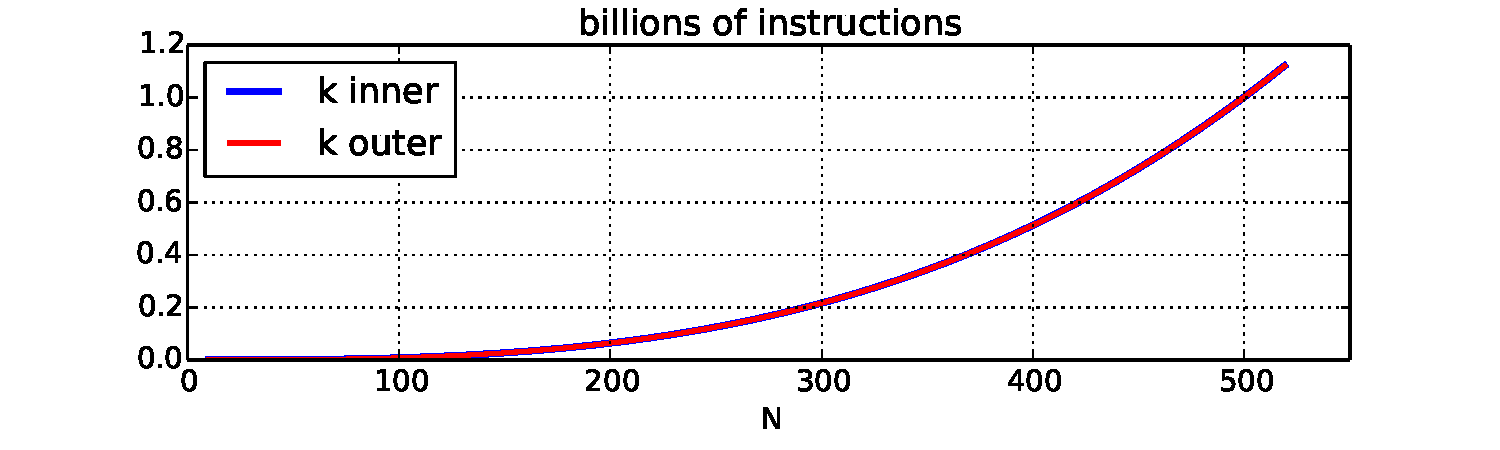
\includegraphics[width=0.99\textwidth]{../caching/k-inout-instrs} \\
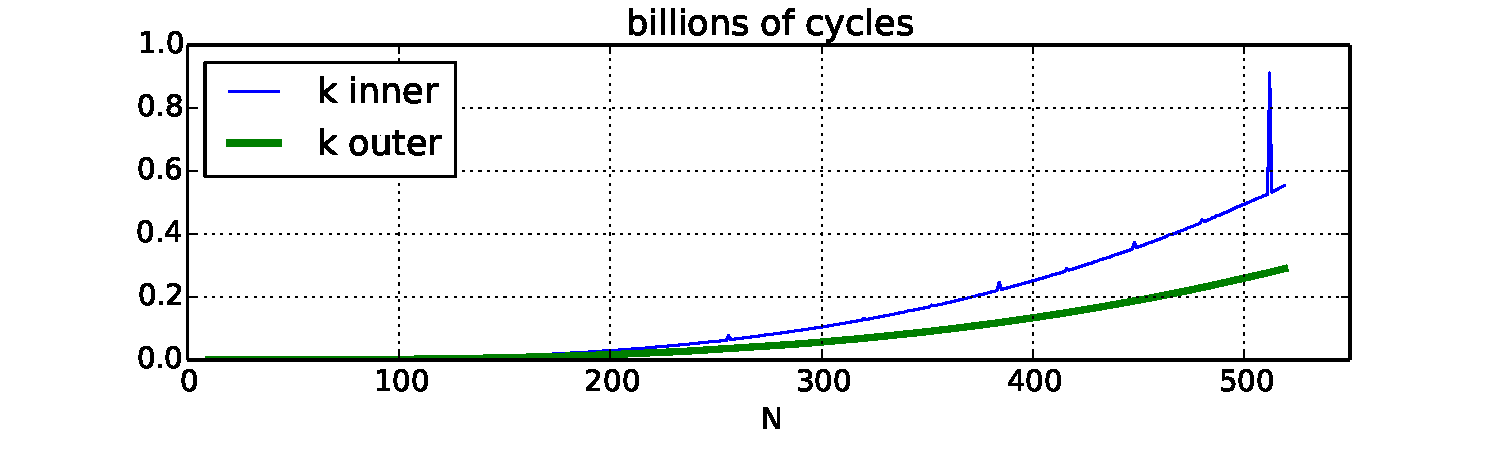
\includegraphics[width=0.99\textwidth]{../caching/k-inout-cycles}
\end{frame}

\begin{frame}{alternate view 1: cycles/instruction}
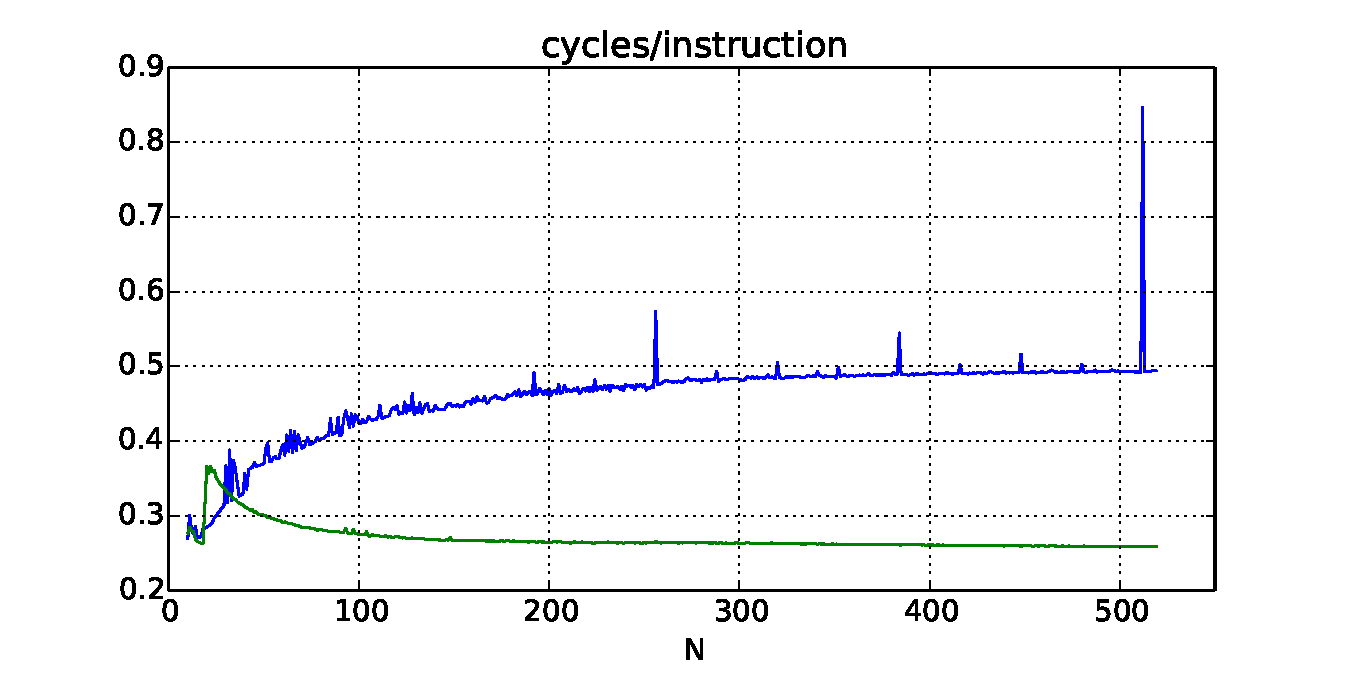
\includegraphics[width=0.99\textwidth]{../caching/k-inout-cpi}
\end{frame}

\begin{frame}{alternate view 2: cycles/operation}
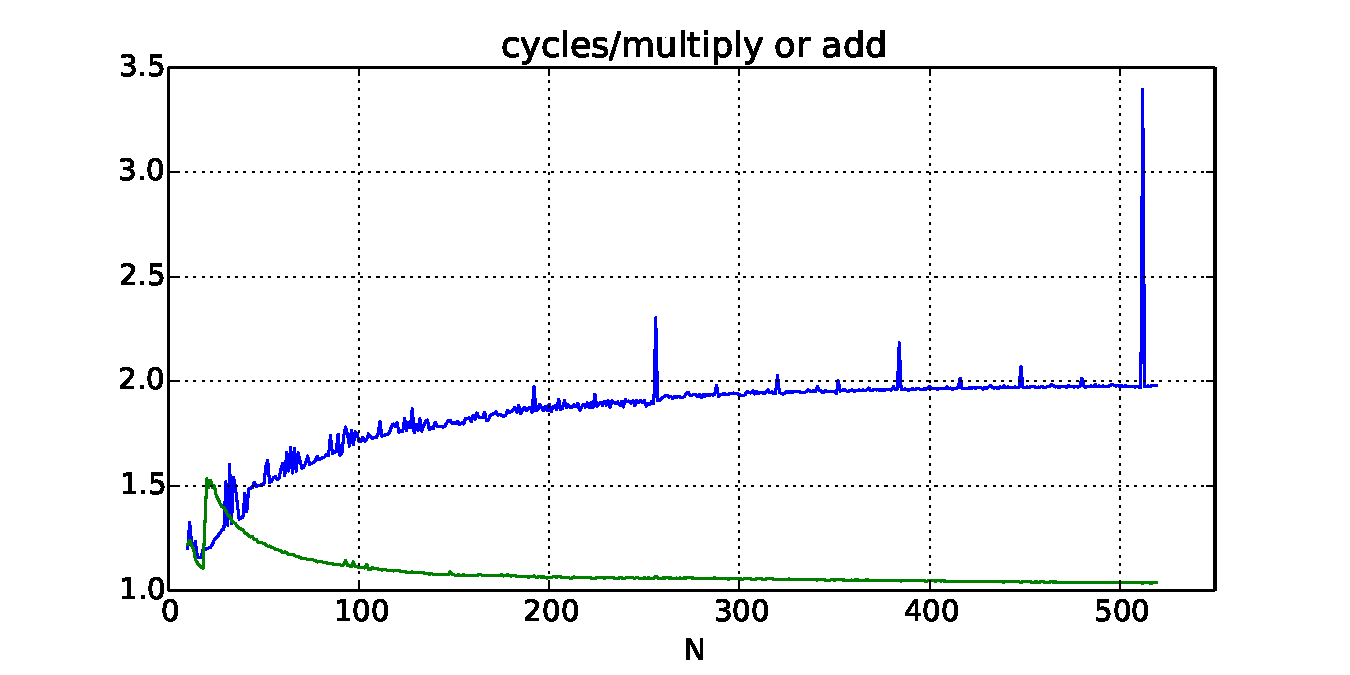
\includegraphics[width=0.99\textwidth]{../caching/k-inout-cpe}
\end{frame}

\begin{frame}{loop orders and locality}
\begin{itemize}
\item loop body: $C_{ij} += A_{ik}A_{kj}$
\item $ki\myemph<2>{j}$ order: $B_{i\myemph<2>{j}}$, $A_{k\myemph<2>{j}}$ have \myemph<1>{spatial locality}
\item $kij$ order: $A_{ik}$ has \myemph<1>{temporal locality}
\item \ldots{} better than \ldots{}
\item $ij\myemph<2>{k}$ order: $A_{i\myemph<2>{k}}$ has spatial locality
\item $ijk$ order: $B_{ij}$ has temporal locality
\end{itemize}
\end{frame}

\begin{frame}[fragile,label=matrixSquareTwoVersionsHilite]{matrix squaring}
\[ B_{ij} = \sum_{k=1}^n A_{ik}\times A_{kj} \]
\lstset{
    style=small,
    language=C,
    moredelim=**[is][\btHL<2>]{~2}{~},
    moredelim=**[is][\btHL<3>]{~3}{~},
    moredelim=**[is][\btHL<4>]{~4}{~},
}
\begin{lstlisting}
/* version 1: inner loop is k, middle is j*/
for (int i = 0; i < N; ++i)
  for (int j = 0; j < N; ++j)
    for (int k = 0; k < N; ++k)
      ~3B[i*N+j]~ += A[i * N + ~2k~] * A[k * N + j];

/* version 2: outer loop is k, middle is i */
for (int k = 0; k < N; ++k)
  for (int i = 0; i < N; ++i)
    for (int j = 0; j < N; ++j)
      B[i*N+~2j~] += ~3A[i * N + k]~ * A[k * N + ~2j~];
\end{lstlisting}
\end{frame}

\begin{frame}{L1 misses}
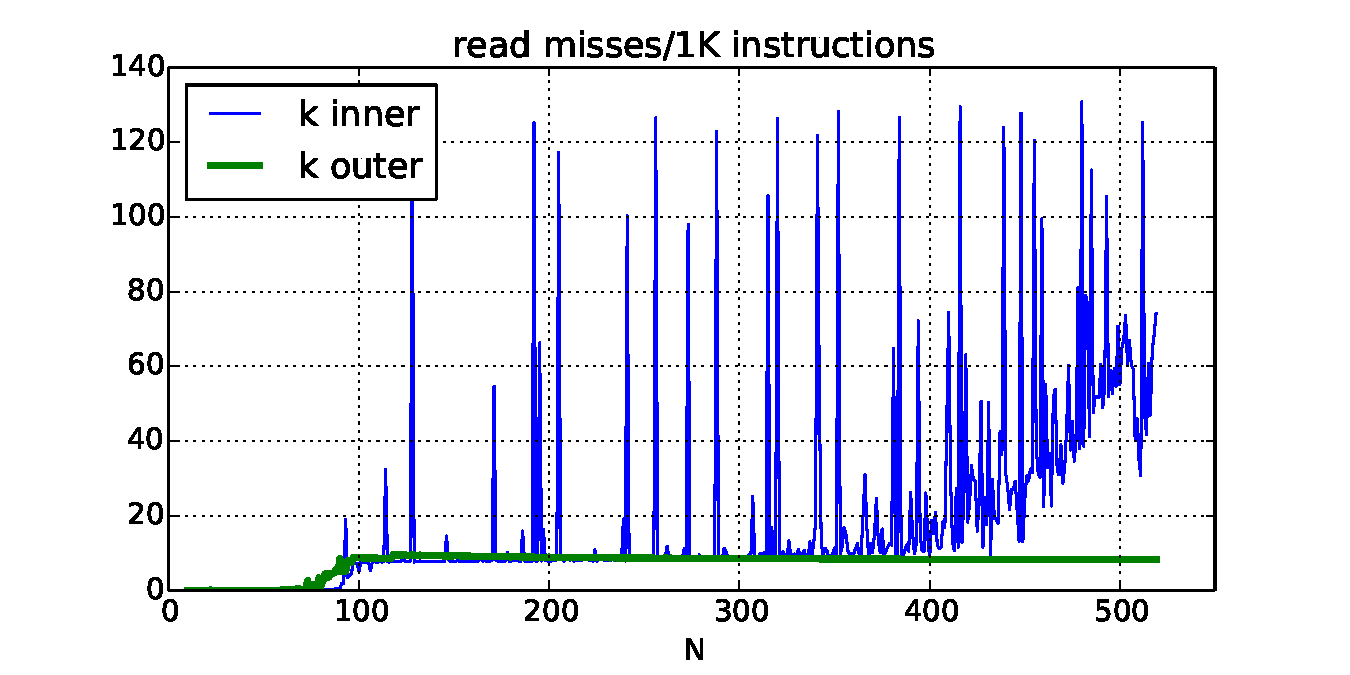
\includegraphics[width=0.99\textwidth]{../caching/k-inout-l1d_read_miss_rate}
\end{frame}

\begin{frame}{L1 miss detail (1)}
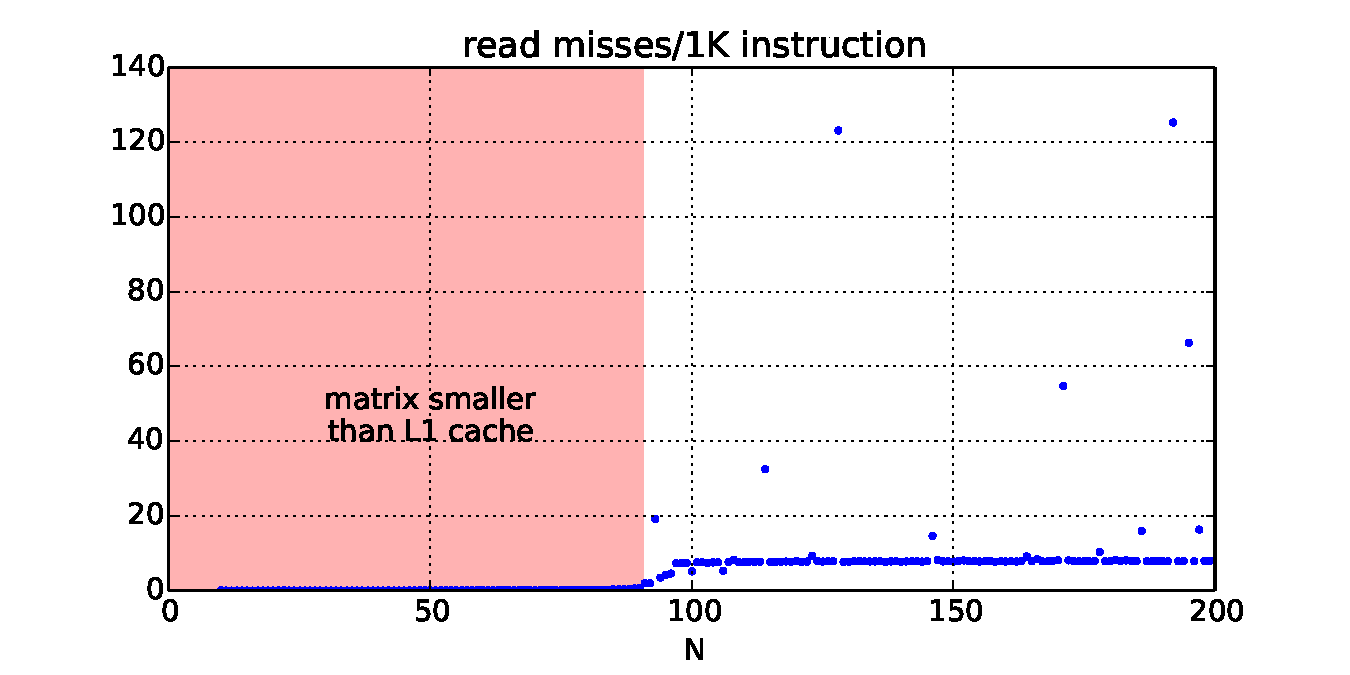
\includegraphics[width=0.99\textwidth]{../caching/k-in-l1d-miss-annot-size}
\end{frame}

\begin{frame}{L1 miss detail (2)}
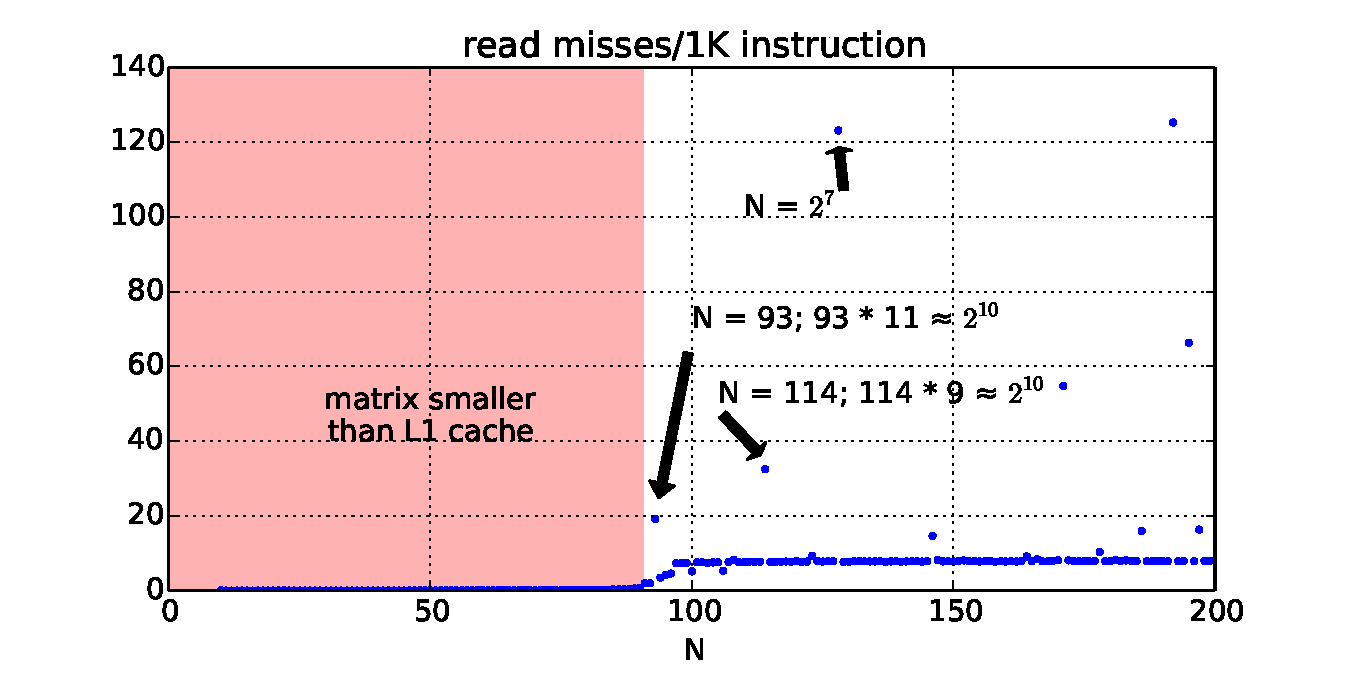
\includegraphics[width=0.99\textwidth]{../caching/k-in-l1d-miss-annot4-size}
\end{frame}

\begin{frame}[fragile,label=conflictExplainPre]{addresses}
    \begin{tabular}{lll}
        \lstinline|A[k*114+j]| &is at& \texttt{10 \textcolor<2>{blue!70!black}{\textbf<2>{0000 00}}00 0100} \\
        \lstinline|A[k*114+j+1]| &is at& \texttt{10 \textcolor<2>{blue!70!black}{\textbf<2>{0000 00}}00 1000} \\
        \lstinline|A[(k+1)*114+j]| &is at& \texttt{10 \textcolor<2>{blue!70!black}{\textbf<2>{0011 10}}01 0100} \\
        \lstinline|A[(k+2)*114+j]| &is at& \texttt{10 \textcolor<2>{blue!70!black}{\textbf<2>{0101 01}}01 1100} \\ 
        \ldots && \\
        \lstinline|A[(k+9)*114+j]| &is at& \texttt{11 \textcolor<2>{blue!70!black}{\textbf<2>{0000 00}}00 1100} \\
    \end{tabular}
    \vspace{.5cm}
    \begin{itemize}
\item<2> recall: \textcolor<2>{blue!70!black}{6 index bits}, 6 block offset bits (L1)
\end{itemize}

\end{frame}


\begin{frame}[fragile,label=conflictExplain]{conflict misses}
\begin{itemize}
\item powers of two --- lower order bits unchanged
\item \lstinline|A[k*93+j]| and \lstinline|A[(k+11)*93+j]|:
    \begin{itemize}
        \item \myemph{1023 elements apart} (4092 bytes; 63.9 cache blocks)
    \end{itemize}
\item 64 sets in L1 cache: usually maps to same set
\item \lstinline|A[k*93+(j+1)]| will not be cached (next $i$ loop)
\item even if in same block as \lstinline|A[k*93+j]|
\end{itemize}
\end{frame}

\begin{frame}{reasoning about loop orders}
    \begin{itemize}
    \item changing loop order changed locality
        \vspace{.5cm}
    \item how do we tell which loop order will be best?
        \begin{itemize}
        \item besides running each one?
        \end{itemize}
    \end{itemize}
\end{frame}

\begin{frame}[fragile,label=cacheBlockMotivation]{systematic approach (1)}
\lstset{style=small,language=C}
\begin{lstlisting}
for (int k = 0; k < N; ++k)
  for (int i = 0; i < N; ++i)
    for (int j = 0; j < N; ++j)
      B[i*N+j] += A[i*N+k] * A[k*N+j];
\end{lstlisting}
\begin{itemize}
\item goal: get most out of \myemph{each cache miss}
\item if $N$ is larger than the cache:
\item miss for $B_{ij}$ --- 1 comptuation
\item miss for $A_{ik}$ --- $N$ computations
\item miss for $A_{kj}$ --- 1 computation
\item effectively caching \myemph{just 1 element}
\end{itemize}
\end{frame}



\begin{frame}{keeping values in cache}
    \begin{itemize}
        \item can't \textit{explicitly} ensure values are kept in cache
        \item \ldots but reusing values \textit{effectively} does this
            \begin{itemize}
                \item cache will try to keep recently used values
            \end{itemize}
            \vspace{.5cm}
        \item cache optimization ideas: choose what's in the cache
            \begin{itemize}
            \item for thinking about it: load values explicitly
            \item for implementing it: access only values we want loaded
            \end{itemize}
    \end{itemize}
\end{frame}
 % FIXME: really before arrays and blocks?

\begin{frame}[fragile,label=arraysAndBlocks]{`flat' 2D arrays and cache blocks}
    \begin{tikzpicture}
    \begin{scope}[x=1.25cm,y=1.25cm]
        \begin{scope}[every node/.style={font=\small\tt}]
            \draw[fill=yellow!50!orange] (0, 5) rectangle (2.7, 4.8);
            \draw[fill=yellow!80!black] (2.7, 5) rectangle (5.4, 4.8);
            \draw[fill=yellow!50!green] (5.4, 5) rectangle (8.1, 4.8);
            \node[anchor=north] at (4, 4.8) {A[N]};
            \node[anchor=north] at (0, 4.8) {A[0]};
        \end{scope}

    \draw[fill=yellow!5] (0, 0) rectangle (4, 4);
    \draw[ultra thick] (4, 0) -- (4, -.1);
    \node[anchor=north] at (0, -.1) { $A_{x0}$ };
    \node[anchor=north] at (4, -.1) { $A_{xN}$ };
    \foreach \y in {3.8} {
        \draw[fill=yellow!50!orange] (0, \y) rectangle ($(2.7, \y) + (0, 0.2)$);
        \draw[fill=yellow!80!black] (2.7, \y) rectangle ($(4.0, \y) + (0, 0.2)$);
    }
    \foreach \y in {3.6} {
        \draw[fill=yellow!80!black] (0, \y) rectangle ($(1.1, \y) + (0, 0.2)$);
        \draw[fill=yellow!50!green] (1.1, \y) rectangle ($(3.8, \y) + (0, 0.2)$);
        \draw[fill=green] (3.8, \y) rectangle ($(4.0, \y) + (0, 0.2)$);
    }
    \foreach \y in {3.4} {
        \draw[fill=green!80!black] (0, \y) rectangle ($(2.5, \y) + (0, 0.2)$);
        \draw[fill=green!50!blue] (2.5, \y) rectangle ($(4.0, \y) + (0, 0.2)$);
    }
    \foreach \y in {3.2} {
        \draw[fill=green!50!blue] (0, \y) rectangle ($(0.2, \y) + (0, 0.2)$);
        \draw[fill=blue!80!black] (0.2, \y) rectangle ($(2.9, \y) + (0, 0.2)$);
        \draw[fill=blue!50!violet] (2.9, \y) rectangle ($(4.0, \y) + (0, 0.2)$);
    }
    \foreach \y in {3.0} {
        \draw[fill=blue!50!violet] (0.0, \y) rectangle ($(1.6, \y) + (0, 0.2)$);
        \draw[fill=violet] (1.6, \y) rectangle ($(4.0, \y) + (0, 0.2)$);
    }
    \foreach \y in {2.8} {
        \draw[fill=violet] (0.0, \y) rectangle ($(0.3, \y) + (0, 0.2)$);
    }
    \end{scope}
    \end{tikzpicture}
\end{frame}

\input{blockDiag}
\input{loadingCounts}

\input{blockingIntro}
\begin{frame}[fragile,label=cacheBlockBetter]{array usage (better)}
\begin{tikzpicture}
\draw[fill=yellow!10] (0, 0) rectangle (4, 4);
\draw[fill=yellow!10] (5, 0) rectangle (9, 4);
%\fill[green] (0.51, 3.49) rectangle (0.19, 3.81);
\fill[green] (3.49, 0.51) rectangle (3.81, 0.19);
%\fill[red] (0.5, 3.5) rectangle (0.2, 3.8) node[black,midway, above=5pt,fill=none,align=left] {$A_{ik}$ to $A_{i+1,k+1}$};
\fill[red] (3.5, 0.5) rectangle (3.8, 0.2) node[black,midway, above=5pt,fill=none,align=left] {$A_{ik}$ to $A_{i+1,k+1}$};
    \begin{visibleenv}<all:2>
        \draw[thick,blue] (3.0, 0.5) rectangle (3.8, 0.35);
        \draw[thick,blue] (3.2, 0.35) rectangle (4.0, 0.2);
    \end{visibleenv}
%\fill[green] (3.5, 0.0) rectangle (3.8, 4.0) node[black,midway,left,align=right,fill=none] {$A_{k0}$\\to\\$A_{k+1,N}$};
\fill[green] (0.0, 3.5) rectangle (4.0, 3.8) node[black,midway,left,align=right,fill=none] {$A_{k0}$\\to\\$A_{k+1,N}$};
%\fill[red] (3.5, 0.8) rectangle (3.8, 0.9);
\fill[red] (0.8, 3.5) rectangle (0.9, 3.8);
%\fill[green] (5.5, 0.0) rectangle (5.2, 4.0) node[black,midway,right,align=left,fill=none] {$B_{i0}$\\to\\$B_{i+1,N}$};
\fill[green] (5.0, 0.5) rectangle (9.0, 0.2) node[black,midway,right,align=left,fill=none] {$B_{i0}$ to $B_{i+1,N}$};
%\fill[red] (5.5, 0.8) rectangle (5.2, 0.9);
\fill[red] (5.9, 0.5) rectangle (5.8, 0.2);
    \begin{visibleenv}<all:1>
\node[anchor=north,align=left] at (4.5,-0.5) {
    more \myemph{temporal} locality:\\
    $N$ calculations for each $A_{ik}$\\% , $A_{i+1,k}$, $A_{i,k+1}$, $A_{i+1,k+1}$ \\
    $2$ calculations for each $B_{ij}$ (for $k$, $k+1$)\\%, $B_{i+1,j}$ (for $k$, $k+1$) \\
    $2$ calculations for each $A_{kj}$ (for $k$, $k+1$)\\%, $B_{k+1,j}$ (for $i$, $i+1$)
};
    \end{visibleenv}
    \begin{visibleenv}<all:2>
\node[anchor=north,align=left] at (4.5,-0.5) {
    more \myemph{spatial} locality: \\
    calculate on each $A_{i,k}$ and $A_{i,k+1}$ together \\
    both in same cache block --- same amount of cache loads
};
    \end{visibleenv}
\end{tikzpicture}
\end{frame}


\input{blockingGeneral}
\begin{frame}[fragile,label=cacheBlockBlock]{array usage: block}
\begin{tikzpicture}
\draw[fill=yellow!10] (0, 0) rectangle (4, 4);
\draw[fill=yellow!10] (5, 0) rectangle (9, 4);
%\fill[green] (0.5, 1.0) rectangle (1.0, 1.5) node[black,midway,left,fill=none,align=left] {$A_{ik}$ block\\($I\times K$)};
\fill[green] (1.0, 0.5) rectangle (1.5, 1.0) node[black,midway,left,fill=none,align=left] {$A_{ik}$ block\\($I\times K$)};
%\fill[green] (1.0, 3.0) rectangle (1.5, 3.5) node[black,midway,above,align=center,fill=none] {$A_{kj}$ block\\($K\times J$)};
\fill[green] (3.0, 1.0) rectangle (3.5, 1.5) node[black,midway,above,align=center,fill=none] {$A_{kj}$ block\\($K\times J$)};
%\fill[green] (5.5, 3.0) rectangle (6.0, 3.5) node[black,midway,above,align=center,fill=none] {$B_{ij}$ block\\($I\times J$)};
\fill[green] (8.0, 0.5) rectangle (8.5, 1.0) node[black,midway,above,align=center,fill=none] {$B_{ij}$ block\\($I\times J$)};
\begin{visibleenv}<1>
\node[anchor=north,align=left] at (4.5,-1) {
    inner loop keeps ``blocks'' from $A$, $B$ in cache
};
\end{visibleenv}
\begin{visibleenv}<2>
%\fill[orange] (0.7,1.0) rectangle (0.8,1.5);
\fill[orange] (1.0,0.7) rectangle (1.5,0.8);
%\fill[orange] (1.0,3.1) rectangle (1.5,3.2);
\fill[orange] (3.1,1.0) rectangle (3.2,1.5);
%\fill[red] (5.7,3.1) rectangle (5.8,3.2);
\fill[red] (8.1,0.7) rectangle (8.2,0.8);
\node[anchor=north,align=left] at (4.5,-1) {
    $B_{ij}$ calculation uses strips from $A$ \\
    $K$ calculations for one load (cache miss)
};
\end{visibleenv}
\begin{visibleenv}<3>
%\fill[red] (0.7,1.1) rectangle (0.8,1.2);
\fill[red] (1.1,0.7) rectangle (1.2,0.8);
%\fill[orange] (1.1,3.0) rectangle (1.2,3.5);
\fill[orange] (3.0,1.1) rectangle (3.5,1.2);
%\fill[orange] (5.7,3.0) rectangle (5.8,3.5);
\fill[orange] (8.0,0.7) rectangle (8.5,0.8);
\node[anchor=north,align=left] at (4.5,-1) {
    $A_{ik}$ calculation uses strips from $A$, $B$\\
    $J$ calculations for one load (cache miss)
};
\end{visibleenv}
\begin{visibleenv}<4->
\node[anchor=north,align=left] at (4.5,-0.5) {
    (approx.) $KIJ$ fully cached calculations \\
    for $KI+IJ+KJ$ loads \\
    (assuming everything stays in cache)
};
\end{visibleenv}
\end{tikzpicture}
\end{frame}

\begin{frame}{cache blocking efficiency}
\begin{itemize}
\item load $I\times K$ elements of $A_{ik}$: 
    \begin{itemize}
        \item do $>J$ multiplies with each
    \end{itemize}
\item load $K\times J$ elements of $A_{kj}$: 
    \begin{itemize}
        \item do $I$ multiplies with each
    \end{itemize}
\item load $I\times J$ elements of $B_{ij}$:
    \begin{itemize}
        \item do $K$ adds with each
    \end{itemize}
\item bigger blocks --- more work per load!
\item catch: $IK+KJ+IJ$ elements must fit in cache
\end{itemize}
\end{frame}

\begin{frame}{cache blocking rule of thumb}
\begin{itemize}
\item fill the \myemph{most of the cache with useful data}
\item and do as much work as possible from that
\item example: my desktop 32KB L1 cache
\item $I=J=K=48$ uses $48^2\times 3$ elements, or $27$KB.
\item assumption: conflict misses aren't important
\end{itemize}
\end{frame}



\input{blockingDivideAndConquer} % FIXME: earlier?

\begin{frame}{cache blocking performance (big sizes)}
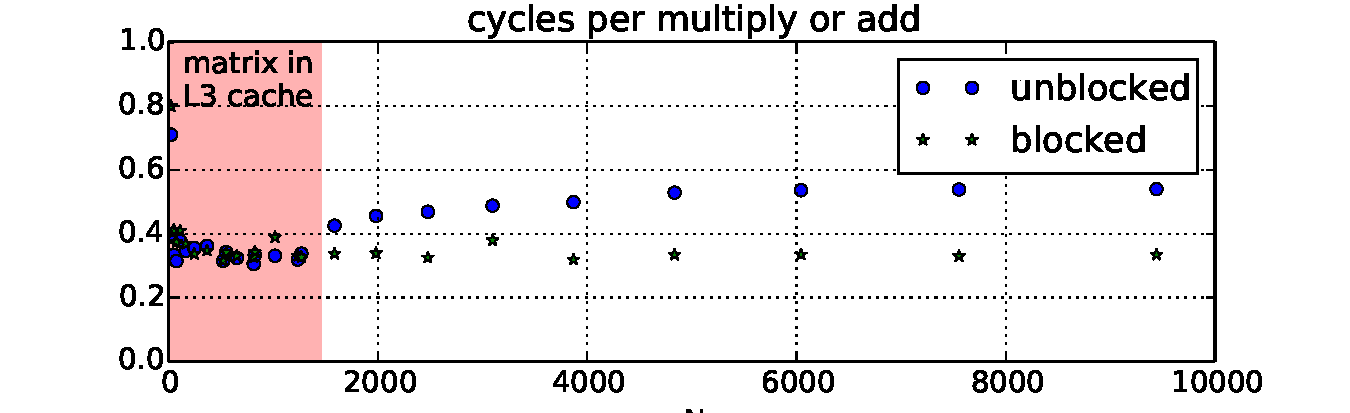
\includegraphics[width=0.99\textwidth]{../optimization/k-vec-big-block-cpelement}
\end{frame}

\begin{frame}{cache blocking performance (small sizes)}
\vspace{-.5cm}
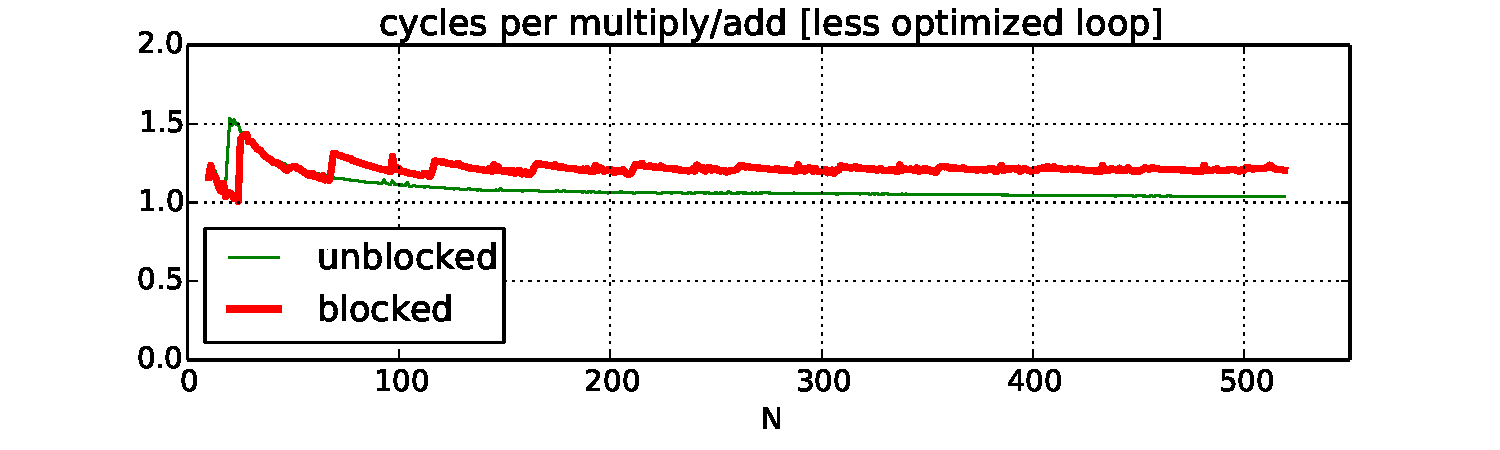
\includegraphics[width=0.8\textwidth]{../optimization/k-block-novec-cyclespercount} \\
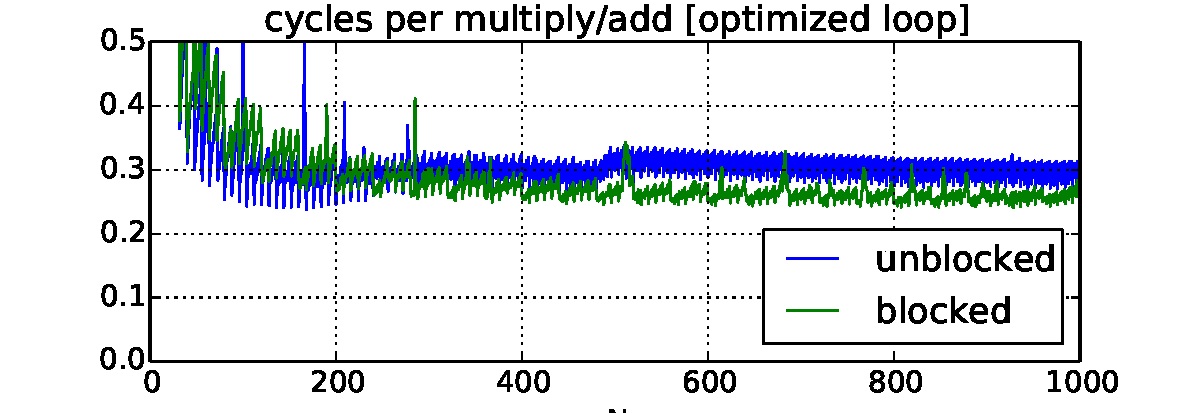
\includegraphics[width=0.8\textwidth]{../optimization/k-blockC-vec-cyclespercount}
\end{frame}

\begin{frame}<1-2>[label=optimizedLoopP]{optimized loop???}
\begin{itemize}
\item performance difference wasn't visible at small sizes 
\item until I optimized \myemph{arithmetic} in the loop
\item (mostly by \myemph<3>{supplying better options to GCC})
\vspace{.5cm}
\item 1: reducing number of loads
\item 2: doing adds/multiplies/etc. with less instructions
\item 3: simplifying address computations
\item<2> but\ldots{} how can that make cache blocking better???
\end{itemize}
\end{frame}

\begin{frame}{overlapping loads and arithmetic}
\begin{tikzpicture}
\draw[thick,-Latex] (0, 0) -- (8,0) node[right] {time};
\begin{scope}[every node/.style={draw}]
\node[overlay,anchor=center,minimum width=3cm,minimum height=1cm] at (-1, -2) {load};
\node[anchor=center,minimum width=7cm,minimum height=1cm] at (5, -2) {load};
\node[overlay,anchor=center,minimum width=3cm,minimum height=1cm] at (12, -2) {load};
\node[overlay,anchor=center,minimum width=3cm,minimum height=1cm] at (0, -3.5) (m0) {multiply};
\node[overlay,anchor=center,minimum width=3cm,minimum height=1cm] at (0, -4.5) (a0) {add};
\node[anchor=center,minimum width=3cm,minimum height=1cm] at (3, -3.5) (m1) {multiply};
\node[anchor=center,minimum width=3cm,minimum height=1cm] at (6, -3.5) (m2) {multiply};
\node[anchor=center,minimum width=3cm,minimum height=1cm] at (9, -3.5) (m3) {multiply};
\node[overlay,anchor=center,minimum width=3cm,minimum height=1cm] at (12, -3.5) (m4) {multiply};
\node[anchor=center,minimum width=3cm,minimum height=1cm] at (3, -4.5) (a1) {add};
\node[anchor=center,minimum width=3cm,minimum height=1cm] at (6, -4.5) (a2) {add};
\node[overlay,anchor=center,minimum width=3cm,minimum height=1cm] at (12, -4.5) (a3) {add};
\end{scope}
\node[fit=(m1) (m2) (m3) (a1) (a2),draw,red,very thick,label={below:speed of load \myemph{might} not matter if these are slower}] {};
\end{tikzpicture}
\end{frame}

\begin{frame}{optimization and bottlenecks}
    \begin{itemize}
        \item arithmetic/loop efficiency was the \myemph{bottleneck}
        \item after fixing this, cache performance was the bottleneck
            \vspace{.5cm}
        \item common theme when optimizing:
            \begin{itemize}
            \item X may not matter until Y is optimized
            \end{itemize}
    \end{itemize}
\end{frame}
 % FIXME: add callback to out-of-order

% FIXME: callback to cache hierarchy
\begin{frame}[fragile,label=registerReuse]{register reuse}
\lstset{style=small,language=C}
\begin{lstlisting}
for (int k = 0; k < N; ++k)
  for (int i = 0; i < N; ++i)
    for (int j = 0; j < N; ++j)
      B[i*N+j] += A[i*N+k] * A[k*N+j];
// optimize into:
for (int k = 0; k < N; ++k)
  for (int i = 0; i < N; ++i) {
    float Aik = A[i*N+k]; // hopefully keep in register!
                          // faster than even cache hit!
    for (int j = 0; j < N; ++j)
      B[i*N+j] += Aik * A[k*N+j];
  }
}
\end{lstlisting}
\begin{itemize}
\item can compiler do this for us?
\end{itemize}
\end{frame}

\begin{frame}[fragile,label=registerReuseAuto]{can compiler do register reuse?}
\lstset{style=small,language=C}
\begin{itemize}
\item Not easily --- What if \lstinline|A=B|? What if \lstinline|A=&B[10]|
\end{itemize}
\begin{lstlisting}
for (int k = 0; k < N; ++k)
  for (int i = 0; i < N; ++i) {
    // want to preload A[i*N+k] here!
    for (int j = 0; j < N; ++j) {
      // but if A = B, modifying here!
      B[i*N+j] += A[i*N+k] * A[k*N+j];
    }
  }
}
\end{lstlisting}
\end{frame}


\begin{frame}[fragile,label=blockingAliasing]{aliasing problems with cache blocking}
\lstset{
    style=small,
    language=C
}
\begin{lstlisting}
  for (int k = 0; k < N; k++) {
    for (int i = 0; i < N; i += 2) {
      for (int j = 0; j < N; j += 2) {
        C[(i+0)*N + j+0] += A[i*N+k] * B[k*N+j];
        C[(i+1)*N + j+0] += A[(i+1)*N+k] * B[k*N+j];
        C[(i+0)*N + j+1] += A[i*N+k] * B[k*N+j+1];
        C[(i+1)*N + j+1] += A[(i+1)*N+k] * B[k*N+j+1];
      }
    }
  }
\end{lstlisting}
\begin{itemize}
    \item can compiler keep \lstinline|A[i*N+k]| in a register?
\end{itemize}
\end{frame}



\begin{frame}[fragile,label=registerBlocking]{``register blocking''}
\lstset{
    style=small,
    language=C
}
\begin{lstlisting}
  for (int k = 0; k < N; ++k) {
    for (int i = 0; i < N; i += 2) {
      float Ai0k = A[(i+0)*N + k];
      float Ai1k = A[(i+1)*N + k];
      for (int j = 0; j < N; j += 2) {
        float Bkj0 = B[k*N + j+0];
        float Bkj1 = B[k*N + j+1];
        C[(i+0)*N + j+0] += Ai0k * Bkj0;
        C[(i+1)*N + j+0] += Ai1k * Bkj0;
        C[(i+0)*N + j+1] += Ai0k * Bkj1;
        C[(i+1)*N + j+1] += Ai1k * Bkj1;
      }
    }
  }
\end{lstlisting}
\end{frame}




\begin{frame}{cache blocking: summary}
\begin{itemize}
\item reorder calculation to reduce cache misses:
\item make \myemph{explicit choice} about what is in cache
\item perform calculations in \myemph{cache-sized blocks}
\item get more spatial and temporal locality
\item temporal locality --- \myemph{reuse values} in many calculations
    \begin{itemize}
    \item before they are replaced in the cache
    \end{itemize}
\item spatial locality --- use \myemph{adjacent values} in calculations
    \begin{itemize}
    \item before cache block is replaced
    \end{itemize}
\end{itemize}
\end{frame}


\begin{frame}[fragile,label=fringeCode1]{cache blocking ugliness --- fringe}
\lstset{
    style=small,
    escapechar=@
}
\begin{lstlisting}
for (int kk = 0; kk < N; kk += K) {
  for (int ii = 0; ii < N; ii += I) {
    for (int jj = 0; jj < N; jj += J) {
      for (int k = kk; k < @\myemph{$\mathtt{\min}(kk+K,N)$}@; ++k) {
          // ...
      }
    }
  }
}
\end{lstlisting}
\end{frame}

\begin{frame}[fragile,label=fringeCode2]{cache blocking ugliness --- fringe}
\lstset{
    style=small,
    escapechar=@
}
\begin{lstlisting}
for (kk = 0; kk + K <= N; kk += K) {
  for (ii = 0; ii + I <= N; ii += I) {
    for (jj = 0; jj + J <= N; ii += J) {
      // ...
    }
    for (; jj < N; ++jj) {
      // handle remainder
    }
  }
  for (; ii < N; ++ii) {
    // handle remainder
  }
}
for (; kk < N; ++kk) {
  // handle remainder
}
\end{lstlisting}
\end{frame}

\begin{frame}[fragile,label=noConflict]{avoiding conflict misses}
\begin{itemize}
\item problem --- array is scattered throughout memory
\item observation: 32KB cache can store 32KB contiguous array
    \begin{itemize}
    \item contiguous array is \myemph{split evenly} among sets
    \end{itemize}
\item solution: \myemph{copy block into contiguous array}
\end{itemize}
\end{frame}

\begin{frame}[fragile,label=noConflictCopy]{avoiding conflict misses (code)}
\begin{lstlisting}[style=small]
process_block(ii, jj, kk) {
  float B_copy[I * J];
  /* pseudocode for loop to save space */
  for i = ii to ii + I, j = jj to jj + J:
    B_copy[i * J + j] = B[i * N + j];
  for i = ii to ii + I, j = jj to jj + J, k:
    B_copy[i * J + j] += A[k * N + j] * A[i * N + k];
  for all i, j:
    B[i * N + j] = B_copy[i * J + j];
}
\end{lstlisting}
\end{frame}


\end{comment}
